\chapter{营养缺乏病}

人类的健康离不开营养,合理的营养能够促进健康,减少疾病。如较长时期营养摄入不足或营养摄入不平衡会导致营养性疾病的发生,有些营养素虽然人体需要的量很少,仅以微克或毫克计算,但缺乏后对人体造成的危害是极其严重的。营养不良(malnutrition)或营养缺乏病(nutritional
deficiency)与长期食物缺乏或饮食中营养素的缺乏有关,社会经济、环境和文化等因素可影响营养缺乏病的流行。营养不良或营养缺乏病将影响儿童和青少年的生长发育,以及人类的智力、行为、学习、工作能力等,而较好的营养状况则能促进儿童和青少年的生长发育,增强人们的体质和有效地提高劳动生产率。

\hypertarget{text00003.htmlux5cux23mllj1}{%
\section{ 概 述}\label{text00003.htmlux5cux23mllj1}}

\hypertarget{text00003.htmlux5cux23mllj2}{%
\subsection{定义}\label{text00003.htmlux5cux23mllj2}}

广义上营养不良包括营养低下(under-nutrition)和营养过剩(over-nutrition)。长期膳食中缺乏一种或多种营养素可导致营养低下,严重营养低下并出现相应临床表现或病症者,则为营养缺乏病,如碘、维生素A、铁等摄入不足将分别会引起地方性甲状腺肿、维生素A缺乏病、贫血等营养缺乏病。营养缺乏病既包括蛋白质能量营养不良(proteinenergy malnutrition,
PEM),也包括特定的营养素缺乏(nutrient
deficiency)。近年来,由于对营养素功能检查日趋完善,各种亚临床的营养缺乏也开始受到重视,因此营养缺乏病也包括亚临床营养缺乏状态。营养过剩则是指由于食物与营养物质过量摄入超过了机体的生理需要而在体内过多积累所引起的一些病症,如肥胖病和其他一些不良代谢性病症。

\hypertarget{text00003.htmlux5cux23mllj3}{%
\subsection{流行病学}\label{text00003.htmlux5cux23mllj3}}

营养不良是全球性公共卫生问题,包括发达国家和发展中国家。然而营养缺乏病大多发生在发展中国家。发展中国家人口约占世界总人口的70%,但食物产量只占世界总产量的40%。2005年世界卫生组织(WHO)报道尼日尔由于自然灾害已造成32000名儿童处于严重营养不良,其中一半已处于危险状态。1997年肯尼亚2~5岁儿童8%存在严重营养不良。在泰国1991年低出生体重儿占9%,1990年学龄期儿童和孕妇缺铁性贫血的发生率分别为18.6%和18.8%。2002年我国营养调查发现5岁以下儿童发育迟缓率仍高达14.3%,其中城市儿童发育迟缓率为4.9%,农村则高达17.3%。我国5岁以下儿童体重低下率为7.8%,其中城市为3.1%,农村为9.3%。同期2岁以内婴幼儿的贫血发生率高达24.2%。1990~1992年,WHO对儿童生长的全球性资料分析结果显示拉丁美洲的洪都拉斯、圭亚那、海地等国家,亚洲南部和东南部,以及非洲西部和东部地区国家的低体重儿童发生率均较高。尤其是学龄前儿童营养不足非常普遍,儿童发育不良和消瘦的全球性地理分布与低体重儿童分布相似,亚洲多数国家儿童发育不良和消瘦发生率高于拉丁美洲,非洲儿童发育不良的趋势与拉丁美洲相似,而消瘦高于亚洲。成人营养状况的资料则显示拉丁美洲国家的成人体质指数(body
mass index,
BMI)<18.5的人口比例在减少,>25的趋势在增加。在非洲,沙漠地区国家较热带和亚热带国家的营养不良的人口比例为大,亚洲国家特别是亚洲南部国家成人BMI<18.5的人口仍占有较大比例,1989~1990年中国营养不良的比例为12.5%,印度为48.6%。2002年中国全国营养调查显示贫血现象仍然比较严重,平均贫血患病率为15.2%,其中城市男性10.6%、女性17.0%,农村男性12.9%、女性18.8%。同样也发现我国成年人超重率已明显上升至22.8%。

\hypertarget{text00003.htmlux5cux23mllj4}{%
\subsection{分类}\label{text00003.htmlux5cux23mllj4}}

营养缺乏病分类可根据不同人群分为儿童、青少年、成人及老年营养缺乏病。按发生原因可分为原发性营养不良(primary
malnutrition)和继发性营养不良(secondary
malnutrition)。前者被认为是由于饮食中营养素摄入不足引起的;后者是在食物或营养素供应正常情况下,由多种因素干扰了机体对营养素的利用发生了障碍而引起的营养缺乏病。

(一)按人群分类

{1.儿童营养缺乏病}
 儿童营养缺乏病是以儿童生长发育减缓为特征,其结果是体重的增长与年龄的增长不成比例。身高和体重的测量是评价儿童营养状况的最常用指标,判断儿童健康和营养状况的最好方法是评价其生长发育。美国CDC在2000年、WHO在2003年均已重新制定了最新评价儿童生长发育的量表,量表中的指标包括有不同性别的年龄别身高、年龄别体重、身高别年龄、年龄别BMI的百分位和Z值评分标准。

{2.青少年营养缺乏病}
 青少年时期身高、体重均快速增加,大约人体的1/4身高是在青少年时期冲刺性达到的。青少年时期是人类一生中很关键的阶段,此期身体的变化程度、成熟程度不仅受基因决定,而且环境因素对其影响也是不小的,如营养不良、感染和慢性疾病均可不同程度的影响青少年的生长发育。此阶段评价发育不良的指标是身高别年龄。

{3.成人营养缺乏病}
 在成人期,营养不良诊断的最简便的方法是BMI。成人的BMI<18.5被认为是慢性营养不良,该标准既适合于男性,也适用于女性。

{4.老年人营养缺乏病}
 60岁以上的老年人口在全球呈现快速增长的趋势,我国于2004年已进入老龄化国家。已证实老年人随着年龄的增长而身高下降,体重也下降。因此,BMI也适用于老年人,可作为老年人群的营养状况、发病和死亡危险的评价指标。我国老年人BMI评价标准目前与成年人相同,<18.5为低体重,>24表示超重。

(二)按发生原因分类

{1.原发性营养缺乏病}
 单纯由营养素摄入减少而引起的一系列异常的临床表现,也可称为饮食性营养缺乏病。主要是因饮食中某种营养素数量不足或者质量不好所致。例如,营养丰富的食品供给不够,或计划不周、调配不好;或者是不良饮食习惯,如偏食、挑食可减少某些营养素的摄取;或者是食物加工过分精细,使某些营养素丢失和破坏过多,如米面加工过度,使维生素B\textsubscript{1}
损失90%,维生素B\textsubscript{2} 、维生素PP和铁损失达70%~85%。

{2.继发性营养缺乏病}
 也称为条件性营养缺乏病,因某种原因引起营养素摄取、吸收和利用障碍,或各种应激因素导致某些营养素需要量增加所致。主要有:①食物摄取功能障碍,如胃肠疾病、神经精神病、食欲减退、食物过敏反应、牙齿脱落和早期妊娠反应等;②营养吸收障碍,如胃肠蠕动过剧、手术切除后吸收面积减少、胃酸和胆汁减少,尤其是阻塞性黄疸;③营养素利用障碍,如肝脏功能异常、糖尿病、甲状腺功能障碍、癌症、放射治疗,或长期服用磺胺类药物等;④特殊情况,如重体力劳动、特殊气候条件和特种作业等。

(三)按营养素缺乏分类

{1.蛋白质-能量营养不良}  蛋白质-能量营养不良(protein-energy
malnutrition,
PEM)是因食物供应不足或因某些疾病等因素而引起的一种营养不良,在世界各地都有发生。因食物供应不足所引起的原发性蛋白质-能量营养不良多发生在饥饿、战争时期或贫困国家和地区的人群;因疾病等因素所引起的继发性蛋白质-能量营养不良则散发在世界各地的患病人群中。蛋白质-能量营养不良在临床上可表现为消瘦型(marasmus)、水肿型(kwashiorkor)及混合型(marasmus-kwashiorkor)3种。消瘦性营养不良是由于长期在膳食中缺乏能量、蛋白质及其他营养素的结果,水肿型营养不良是由于膳食中蛋白质严重缺乏而能量的供给尚可维持最低水平的极度营养不良症。大多数病人的临床表现为混合型。

{2.维生素缺乏}
 由于维生素缺乏引起的各种缺乏病,常见的主要有:维生素A缺乏引起的夜盲、角膜软化、干眼病,维生素B\textsubscript{1}
缺乏引起的脚气病,维生素B\textsubscript{2}
缺乏引起的皮肤损害,维生素C缺乏引起的坏血病,以及叶酸和维生素B\textsubscript{12}
缺乏引起的恶性贫血等。

{3.无机盐缺乏}
 无机盐缺乏引起的营养缺乏病常见的主要有:缺碘引起的甲状腺肿或克汀病,缺铁引起的小细胞低色素性贫血,缺钙引起的软骨病,缺硒引起的克山病等。

\hypertarget{text00003.htmlux5cux23mllj5}{%
\subsection{病因}\label{text00003.htmlux5cux23mllj5}}

(一)营养素摄入不足

最常见的是食物摄入不足,其原因可以是原发性的,也可以是继发性的。

原发性摄入不足中,因自然灾害或战争等社会因素引起的食物短缺常常表现为蛋白质-能量营养不良为主。在正常情况下,水质和土质中缺少某种营养素,或偏食等可引起某种营养素缺乏,有时某地区人群的生活习惯性偏食甚至可导致某种营养素缺乏病的流行。食物因加工烹调不合理而破坏了营养素,尽管食物摄入量并不少,但营养素摄入很少亦可发生营养素缺乏而引起营养素缺乏病,如水溶性维生素的缺乏中,食用精白米面和丢弃米汤常是脚气病的主要原因,蔬菜先切后洗,烫、漂、捞、挤等加工过程将使大部分维生素C遭受破坏而引起坏血病。

食物摄入不足的继发性原因是食欲不振、昏迷、精神失常或神经性厌食、口腔及颔面手术后、食管癌和贲门癌等引起肠胃道梗阻的疾病。在这些疾病中常采用鼻饲或静脉营养补给措施,但如补给量不能满足病人需要时,仍可产生营养素缺乏的症状。

(二)营养素吸收不良

胃肠道、胰腺和胆道等疾病因一系列消化酶等活性因子分泌障碍将严重影响食物中营养素的消化和吸收。如胆道和胰腺疾患将导致食物中脂肪和脂溶性维生素的吸收受阻;胃肠道不同部位的切除在临床上可产生相应部位吸收的营养素缺乏表现,如回盲部切除可引起叶酸和维生素B\textsubscript{12}
缺乏性贫血,放射性肠炎可引起消化道广泛性的吸收不良。有些药物可阻止营养素的吸收,或影响营养素代谢而致主动运输机制受到抑制,如石蜡油溶解脂溶性维生素而造成吸收不良,新霉素和秋水仙素造成绒毛的结构缺陷和酶的损害,使脂肪、乳糖、维生素B\textsubscript{12}
、无机盐等吸收不良,消胆剂通过与胆盐结合而降低胆固醇,将继发因胆盐缺乏而致的吸收不良。长期服用抗惊厥药或双磷酸酯类可影响钙的吸收,但其机制不同,前者是由于加速维生素D\textsubscript{3}
及其活性代谢物的分解代谢,而后者是由于1,25-(OH)\textsubscript{2}
D\textsubscript{3}
的形成减少。另外,还有先天性缺陷造成的,如先天性维生素B\textsubscript{12}
吸收不良,其缺陷在于维生素B\textsubscript{12}
被吸收后缺乏运输的球蛋白,须依赖肌注球蛋白才能维持血象正常。

近年证明营养素之间的不平衡也是造成吸收不良的因素。对防治心血管疾病和肠道肿瘤有好处的膳食纤维如摄入过多将影响无机盐的吸收,而无机盐之间,如铁和锌相互间须保持一定比例,如一方过高即引起另一方的吸收减少。

(三)营养素利用减少

常见的是肝脏疾病使营养素的利用率或储备能力下降,肝硬化时常合并维生素A、维生素B\textsubscript{6}
、维生素B\textsubscript{12}
、叶酸的储存减少而出现缺乏。尿毒症时肾脏不能使25-OH---D\textsubscript{3}
转变为活性形式的1,25-(OH)\textsubscript{2} D\textsubscript{3}
,导致肠道吸收钙的障碍。有的是由于其性质是营养素的拮抗剂,故在作为药物使用时可抑制营养素的功用,如抗肿瘤药脱氧吡哆醇是维生素B\textsubscript{6}
的同系物,能抑制需要维生素B\textsubscript{6}
的酶系。又如高剂量的异烟肼或肼苯哒嗪均可引起维生素B\textsubscript{6}
的缺乏,均属于拮抗维生素B\textsubscript{6}
的作用所致。有少数也可能是遗传性疾病引起的利用有缺陷,如肝细胞中先天性缺少亚胺甲基转移酶或N-5甲基四氢叶酸转换酶活力减低导致叶酸利用缺陷。维生素B\textsubscript{6}
的遗传性缺陷是由于酶蛋白的缺陷而影响维生素B\textsubscript{6}
与辅酶的结合,表现出婴儿惊厥、贫血、高胱氨酸尿等维生素B\textsubscript{6}
反应性疾病。

(四)营养素损耗增加

长期发热,代谢功能亢进及各种癌症,其他消耗性疾病如糖尿病、结核病均明显地增加体内各种物质的消耗。创伤、大手术、大面积烧伤等促使组织分解代谢加剧的情况,使大量氮从尿中及创面丢失,代谢率也显著增加。消化道瘘、肾脏病也是蛋白质丢失较多并容易发生营养缺乏的疾病。放疗或化疗造成的营养素损耗及蛋白质合成障碍如不及时补给满足需要,常使病人的周身情况变得虚弱,影响治疗效果。寄生虫疾病在第三世界比较普遍,营养缺乏的原因与寄生虫感染引起的营养素损耗增加有关。长期的慢性失血也应该及时治疗,从而防止营养缺乏病的发生。总之,一切引起代谢加速及营养素丢失的疾患都应密切注意,及早治疗。

(五)营养素需要增加

在人体生长发育旺盛及妊娠、哺乳等生理过程中,营养需要量有明显的增加。如细胞分裂时核酸合成增加,其中叶酸是必不可少的营养素,因而在妊娠的初期必须增加叶酸需要量以适应胎儿组织生长发育的需要。到妊娠后期胎儿成熟,体内要有一定的营养素储备,此时母体对蛋白质的需要量必然增加,如营养供给不足则使胎儿生长缓慢,骨骼或脑的成熟过程可能发生障碍。乳母为了保证乳汁的分泌量和其营养成分,各种营养素的需要量都要有明显增加。此时,如果有营养素吸收不良、利用减少和损耗增加的情况,则更容易发生营养缺乏。因此,对于这一类人群,更要注意营养缺乏病的防治。

\hypertarget{text00003.htmlux5cux23mllj6}{%
\subsection{诊断}\label{text00003.htmlux5cux23mllj6}}

营养缺乏病的诊断依赖于膳食史、体格检查、生化检查和治疗试验。

(一)膳食史

了解膳食摄取情况最精确的方法是称重法膳食调查,即对每餐食物烹调前后和剩余量都进行称重,然后折合每天实吃的各种食物重量,查食物成分表,算出每天热能和营养素的摄取量。这种方法大多用于集体调查,对个体病人似乎过于繁琐。有经验的营养师及临床医师询问了解病人的膳食习惯及每天的摄取量就能基本上判断各类营养素是否缺乏。如能取得病人及家属的配合,记录3天的摄入食物量,则以此计算所得的数据,核对询问结果,更加可靠。

(二)体格检查

体格检查常用来评价儿童生长发育和营养状况,最常使用的人体测量指标有身高和体重。评价儿童生长发育的量表有不同性别的年龄别体重、年龄别身高、身高别年龄、年龄别BMI的百分位和Z值评分标准。我国参照WHO关于儿童营养不良体格测量的评估标准如下:①体重低下(underweight)是指按年龄别体重法,与同年龄、同性别正常参照值相比,此指标反映儿童过去和(或)现在有慢性和(或)急性营养不良,但单凭此项不能区别急性还是慢性营养不良;②生长迟缓(stunting)是指按年龄别身高法,与同年龄、同性别正常参照值相比,此指标主要反映过去或长期慢性营养不良;③消瘦(marasmus)是指按身高别体重法,与同年龄、同性别正常参照值相比,此指标反映儿童近期急性营养不良。而儿童与青少年超重和肥胖的评价标准通常采用年龄别BMI法。成人的营养状况评价目前通常采用BMI,国内标准为:BMI<18.5为营养不良,18.5~23.9为正常,≥24为超重,≥28为肥胖。

(三)临床表现

营养缺乏病的临床症状有特异性和非特异性两大类。根据病人的脸色、体重、精神状态可以对其营养状态有一个初步估计。然后,根据机体主要受影响部位的检查,如头发、眼、唇、口腔和皮肤,进一步确定何种营养素的缺乏。

{1.头发}
 蛋白质-能量营养不良可使头发颜色变为灰暗,变细、干、脆,营养严重缺乏时头发极易脱落,发根容易断裂。

{2.眼}
 维生素A缺乏引起干眼病,开始时球结膜干燥,失去光泽,泪液减少,进一步角膜软化,引起溃疡、穿孔和破坏,最终留下灰白色角膜瘢痕,完全失明。

{3.口腔}
 口腔是营养缺乏的最敏感部位,但其表现是非特异性的。如缺铁性贫血和巨幼红细胞性贫血在口唇和口腔黏膜部位都出现苍白。口角炎是维生素B\textsubscript{2}
缺乏的症状,同时还有舌乳头肥大。维生素C缺乏可使齿龈充血肿胀、易出血。现在已知维生素A、烟酸和核黄素缺乏也可引起齿龈炎,故治疗也应考虑综合措施。

{4.皮肤}
 维生素A缺乏的皮肤症状是毛囊角化,其形状如“鹅皮”,从过度增生的毛囊内突出粗糙的角化丘疹,用手触之如搓板,上臂和大腿外侧处皮肤最为明显。维生素C缺乏也产生毛囊症状,但表现为毛囊周围的充血、肿胀,继而也增生,与维生素A缺乏应相鉴别,特别是常伴有出血点等表现。烟酸缺乏引起癞皮病,典型症状是在暴露部位和压迫处的皮肤增厚、干燥,出现红斑。严重蛋白质缺乏会引起四肢凹陷性水肿和过度角化、过度色素沉着和脱皮为特点的皮炎,其与癞皮病的区别在于不限于暴露部。急性脚气病也有下肢水肿,严重时遍及全身。

{5.颈部}  碘缺乏引起的甲状腺肿以望诊和触诊确定较容易。

{6.神经病变}  许多营养缺乏病都有神经症状,如维生素B\textsubscript{1}
缺乏伴有周围神经性无力和感觉异常,维生素B\textsubscript{6}
缺乏引起婴儿惊厥,维生素B\textsubscript{12}
缺乏可引起脊髓的亚急性退化性变,癞皮病常有精神症状。

(四)生化检查

营养缺乏病的临床症状不仅1种,往往多种合并出现,且同一症状可能是几种营养素缺乏的表现,故鉴别诊断必须依靠生化检查。生化检查方法基本分为下列几种:①测定血液中营养成分的浓度;②测定营养成分经尿排出的速率;③测定血或尿中的营养素的代谢产物;④测定与营养素有关的酶活性的改变;⑤给予大剂量某种营养素后测定其在尿中的排出量,即饱和试验;⑥测定毛发和指甲中的含量。

近年来,在实验室检查中,除了生化测定外,还有免疫功能试验,已证明营养缺乏时机体的免疫功能显著下降。当血清白蛋白<30g/L或实际体重低于理想体重的85%以下,蛋白质-能量营养不良常伴有免疫功能降低,表现有总淋巴细胞计数减少、淋巴细胞对植物血细胞凝集素的反应、中性白细胞的趋化性及迟发性超敏皮试反应均低下。临床上采用简易而有预测价值的总淋巴细胞计数及迟发性超敏皮试作为诊断营养缺乏的指标。

\hypertarget{text00003.htmlux5cux23mllj7}{%
\subsection{治疗原则}\label{text00003.htmlux5cux23mllj7}}

(1)营养素缺乏病的治疗应针对病因。继发性营养素缺乏应注意主要病因的治疗,原发性缺乏也要考虑解除影响摄入不足的因素,为补充食物或营养素创造条件。营养治疗要成为整体治疗方案的组成部分,与其他治疗措施相辅相成,相互促进和补充。

(2)营养缺乏病治疗所采用的补充剂量要适宜,不必使用过高的治疗量或维持量,尤其对于有毒副作用的营养素更应注意。对于不同年龄、不同情况的病人,要区别对待。最好是根据临床症状和生化检查结果来决定。

(3)在营养缺乏病治疗时不能只考虑主要缺乏的营养素,而应全面从各种营养素之间的相互关系来考虑治疗方案,以期达到病人恢复到具有合理营养状况的健康水平。例如对蛋白质营养不良治疗时,除补充蛋白质外,还应相应补充能量和维生素,否则蛋白质不能有效被利用。

(4)营养缺乏病的治疗应循序渐进,如不宜突然用高热能、高蛋白质膳食治疗重度蛋白质-能量营养不良,因机体长期缺乏营养后肠胃道和其他器官的功能处在萎缩和低下状态,不能适应一时的超负荷营养。

(5)营养缺乏病的治疗一般应充分利用食物,配制适合于疾病特点的治疗膳食。当病人摄食困难或神志不清,可考虑管饲肠内营养;当肠内营养仍不能满足需要时,才考虑静脉营养支持。在病人病情好转以后,尽早恢复正常的膳食治疗。

(6)营养缺乏病的治疗一般须坚持一段时间,短期见效缓慢。效果应以病人营养状况的全面恢复、临床与亚临床症候消失、抵抗能力增强等客观指标为依据。

\hypertarget{text00003.htmlux5cux23mllj8}{%
\section{ 蛋白质-能量营养不良}\label{text00003.htmlux5cux23mllj8}}

蛋白质-能量营养不良(protein-energy malnutrition,
PEM)是因为食物中蛋白质和(或)能量供给不足或由于某些疾病等因素而引起的一种营养不良,在世界各地均有发生。主要表现为渐进性消瘦、皮下脂肪减少、水肿及各器官功能紊乱。严重PEM可直接造成死亡,轻型慢性的PEM常被人们忽视,但对儿童的生长发育和疾病康复有很大影响,所以PEM是临床营养学上的重要问题。

\hypertarget{text00003.htmlux5cux23mllj9}{%
\subsection{流行病学}\label{text00003.htmlux5cux23mllj9}}

PEM是发展中国家最常见的营养性疾病。轻、中度PEM的临床表现不如维生素或无机盐缺乏的症状明显,在婴幼儿中,表现为生长迟缓、体格瘦小;严重者易于识别,多呈现极度消瘦或水肿、智力发育迟钝、死亡率高。1990年有关调查显示,根据年龄别体重低于参考值减两个标准差以下者,估计发展中国家5岁以下儿童每3人就有1人,相当于1亿7千7百万儿童患有或曾患有营养不良,其流行范围从美洲的14%到南亚的47%。自1986年开始,在我国7个省选择18个较贫困的地区连续4年对10000名左右的学龄前儿童进行营养状况调查。结果表明,他们主要表现为慢性营养不良,以1~2岁最为严重,儿童生长迟缓和体重低下的发生率分别为12.4%~76.4%和6.9%~44.3%。在2002年第四次全国营养调查中发现我国5岁以下儿童生长迟缓率仍高达14.3%,其中农村儿童生长迟缓现象更高(20.9%)。在住院患儿中,营养不良的发生率也仍居高不下。如上海儿童医学中心在2000年对218例小儿先天性心脏病患儿的营养调查中发现营养不良的发生率为61%。2006年有人对上海3家具有较大儿科规模医院收治的349例先天性幽门肥厚患儿的营养调查显示营养不良率为49.6%。1999~2010年,全球儿童营养不良的情况略有缓解,低体重发生率从26.5%下降至22.4%。亚洲罹患低体重的人数下降最快,从35.1%降至27.9%。然而,尽管这一时期低体重发生率有了显著下降,但是亚洲中南部国家儿童营养不良的情况仍处于极高的水平。

成年人的轻、中度蛋白质-能量营养不良一般不易发觉,但在食物供应不足的地区常有发生。在一般情况下,在少数严重病例发生的地区也常伴有大量亚临床症状的病人存在。在重体力劳动者,如摄取食物不足,难以维持蛋白质-能量平衡,表现为身体虚弱无力,不爱活动,劳动效率下降;妇女则表现为孕期体重增加缓慢,初生儿体重较轻,乳汁分泌量减少。在住院病人中蛋白质-能量营养不良则更加普遍,如美国和英国成人外科病人分别为50%和30%,德国成人内科病人中为51.2%。危地马拉入院病人中的中度蛋白质-能量营养不良占80%,泰国为60.7%~86.6%。中国2005年统计资料显示:全国4个直辖市、5个自治区和19个省共403所医院的蛋白质-能量营养不良在成人外科病人中平均为43%、普内科和神经内科病人中为30%~50%,重症监护病房(ICU)病人中为60%~65%。

\hypertarget{text00003.htmlux5cux23mllj10}{%
\subsection{病因}\label{text00003.htmlux5cux23mllj10}}

根据引起蛋白质-能量缺乏的发病原因分为原发性和继发性两种。

(一)原发性蛋白质-能量营养不良

原发性蛋白质-能量营养不良是因食物中蛋白质和(或)能量的摄入量不能满足身体的生理需要而发生的。其主要原因为饮食不当和摄入不足,如婴儿期母乳不足,而未及时和正确地采用混合喂养;奶粉配制过于稀释;未按时和适当添加辅食;骤然断奶,婴儿不能适应或拒绝新的食品。较大小儿常见不良饮食习惯,偏食或素食,多食糖果,厌食奶类、肉类、蛋类,长期单纯使用淀粉样食品(如奶糕、粥),饮食中长期食物成分搭配不当,能量不够或蛋白质太少。以上原因均可造成摄入不够致蛋白质-能量摄入不足。

(二)继发性蛋白质-能量营养不良

继发性蛋白质-能量营养不良多与疾病有关。主要由于患病后食欲减低、吸收不良、分解代谢亢进、消耗增加、合成代谢障碍所致。多见于消化道感染(如迁延性腹泻、慢性痢疾、严重寄生虫感染等),肠吸收不良综合征,消化道先天性畸形(如唇裂、腭裂、先天性肥厚性幽门狭窄和短肠综合征等),慢性消耗性疾病(如结核、肝炎、长期发热、恶性肿瘤等)等。

\hypertarget{text00003.htmlux5cux23mllj11}{%
\subsection{病理生理}\label{text00003.htmlux5cux23mllj11}}

由于蛋白质和能量供应不足,机体首先动用贮存的糖原,继之动用脂肪,出现脂肪减少,最后动用蛋白质氧化供能,导致机体蛋白质消耗,引起负氮平衡。随着全身脂肪大量消耗和血浆蛋白低下,全身总液体量相对增多,使细胞外液呈低渗性。如有呕吐、腹泻,易出现低渗性脱水和酸中毒,出现低钠、低钾、低镁及低钙血症。重度营养不良对消化系统,心、肾功能,以及中枢神经系统均有影响。

{1.消化系统}
 胃肠黏膜变薄甚至萎缩,上皮细胞变形,小肠绒毛失去正常形态和蠕动。胃酸减低,双糖酶减少。胰腺缩小,胰腺的分泌酶活性降低。肠蠕动减慢,消化吸收功能下降,菌群失调,易引起腹泻。

{2.心脏功能}
 严重病例引起心排血量减少,心率减慢,循环时间延长,外周血流量减少,心电图常常无特异性改变,X线示心脏缩小。

{3.肾功能}
 严重者肾小管细胞浑浊肿胀,脂肪浸润。肾小球滤过率和肾血流量减少,浓缩功能降低,尿比重下降。

{4.中枢神经系统}
 营养不良对大脑和智力发育有很大影响。营养不良如发生在脑发育的高峰期,将影响脑的体积和化学组成,使脑的重量减轻,磷脂减少。表现为想象力、知觉、语言和动作能力落后于正常儿,智商低下。

\hypertarget{text00003.htmlux5cux23mllj12}{%
\subsection{临床表现}\label{text00003.htmlux5cux23mllj12}}

临床上根据体重、皮下脂肪减少的程度和全身症状的轻重将营养不良分为轻度、中度和重度。在临床表现的特征上又可将营养不良分为消瘦型(marasmus)、水肿型(kwashiorkor)、消瘦-水肿型(marasmus-kwashiorkor)、营养性侏儒(nutritional
dwarfing)和体重低下(underweight)等类型。

消瘦型是以消瘦为主要特征。体重明显下降,骨瘦如柴,儿童生长发育迟缓,皮下脂肪减少,皮肤干燥松弛,多皱纹,失去弹性和光泽,头发松稀,失去固有光泽,面若猴腮,体弱无力,缓脉,低血压,低体温,易哭闹。

水肿型是以全身水肿为主要特征。轻者见于下肢、足背;重者见于腰背部、外生殖器及面部。儿童身高可正常,体内脂肪也未见减少,但肌肉松弛,似满月脸,眼睑水肿,易剥落的漆皮状皮肤病,指甲脆弱有横沟,表情淡漠,易激惹和任性,常伴发脂肪肝。

消瘦-水肿型临床表现介于两者之间,病人体重低于标准体重的60%,并伴有水肿。这种情况常呈区域性出现,与膳食缺乏的程度有关,还与社会因素有关。

营养性侏儒体重低于其标准体重的60%,年龄别体重低下,但身高别体重尚可,主要是由于长期蛋白质和能量缺乏,其结果表现为生长迟缓。因身高和体重成比例落后,故表面上看似乎正常。生长期小儿常骨龄滞后。

体重低下是轻度到中度的亚临床蛋白质-能量营养不良表现,病人体重在其标准体重的60%~80%,血浆白蛋白减少,其他与蛋白质缺乏相关的指标也可能改变。

单纯性蛋白质或能量营养不良较少见,多数病例为蛋白质和能量同时缺乏,表现为混合型蛋白质-能量营养不良(按程度分类见表2-1)。

\begin{table}[htbp]
\centering
\caption{蛋白质-能量营养不良(PEM)的分类}
\label{tab2-1}
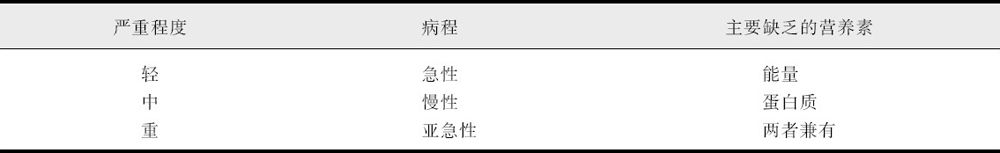
\includegraphics{./images/Image00006.jpg}
\end{table}

\hypertarget{text00003.htmlux5cux23mllj13}{%
\subsection{诊断}\label{text00003.htmlux5cux23mllj13}}

(一)病史

应详细询问喂养和饮食史,采用回顾法了解病人的发病情况与饮食的关系,估算出一日蛋白质和热能的摄入量,对诊断有重要价值。

(二)临床表现

蛋白质-能量营养不良临床上有体重下降、皮下脂肪减少、全身各系统功能紊乱的症状和体征。

(三)体格测量

{1.儿童}  体格测量的指标是评价儿童生长与营养状态的一种简单的测量方法。

(1)体重:体重不增或减轻是最早出现的症状。

(2)年龄别身高:是代表线性生长,本质上是测量长期生长不良的指标。

(3)身高别体重:可反映身体比例或生长协调性,尤其对急性生长障碍特别敏感。

(4)年龄别体重:既代表线性生长又代表身体比例。

1995年“全国提高儿童生命质量学术会议”决定我国也参照WHO关于儿童营养不良体格测量指标的评估标准: ①体重低下(underweight)。根据年龄别体重,与同年龄、同性别正常参照值相比,低于中位数减2SD,但≥中位数减3SD者为中度体重低下;<中位数减3SD者为重度体重低下。此指标反映儿童过去和(或)现在有慢性和(或)急性营养不良,但单凭此项不能区别急性还是慢性营养不良。②生长迟缓(stunting)。按年龄别身高,与同年龄、同性别正常参照值相比,低于中位数减2SD,但≥中位数减3SD者为中度生长迟缓;低于中位数减3SD者为重度生长迟缓。此指标主要反映过去或长期慢性营养不良。③消瘦(marasmus)按身高别体重,与同年龄、同性别正常参照值相比,低于中位数减2SD,但≥中位数减3SD者为中度消瘦;低于中位数减3SD者为重度消瘦。此指标反映儿童近期、急性营养不良。

{2.成人}  体质指数和体重是评价成人健康与营养状态的一种指标。

(1)体质指数(BMI):青少年和成人可用BMI来评价。BMI<18.5为营养不良,BMI<17.5为中度营养不良,BMI<16.5为重度营养不良。

(2)体重改变:由于我国目前尚无统一的标准体重值,故采用体重改变做指标更合理,并将体重变化的幅度与速度结合起来考虑。计算公式为:体重改变(%)=[平时体重(kg)-现时体重(kg)]/平时体重(kg)×100%,其评价标准见表2-2。

\begin{table}[htbp]
\centering
\caption{体重变化的评定标准}
\label{tab2-2}
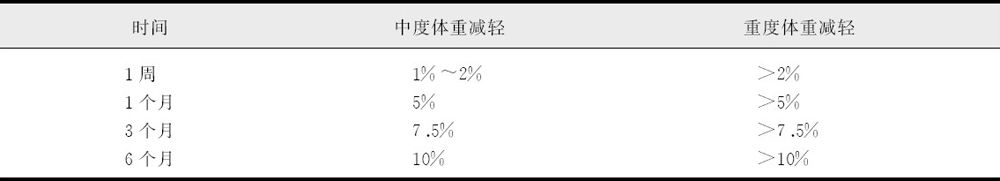
\includegraphics{./images/Image00007.jpg}
\end{table}

(四)实验室检查

蛋白质缺乏病人的血清白蛋白和总蛋白值明显下降,当血浆总蛋白<45g/L、白蛋白<28g/L时会出现水肿,同时血清前白蛋白、血清转铁蛋白和结合蛋白如甲状腺素结合前白蛋白、血浆铜蓝蛋白、视黄醇结合蛋白等也减低。一般情况下其血糖、血胆固醇和血尿素氮、肌酐水平也下降。伴贫血时,血红蛋白和红细胞计数也减少。在肾功能正常时,24小时尿肌酐可作瘦体组织状况评价的指标,尿肌酐/身高指数是评价肌蛋白消耗的指标。免疫指标主要有淋巴细胞总数减少、皮肤延迟超敏反应低下或无反应等现象。

(五)综合评价

PEM是一个复杂的临床综合征,目前尚无简单可靠的方法对各类型,尤其是亚临床类型进行诊断,大多数需根据主要临床症状、人体测量参数和实验室检查数据进行综合评价(表2-3)。

\begin{table}[htbp]
\centering
\caption{人体测量和实验室指标的诊断标准}
\label{tab2-3}
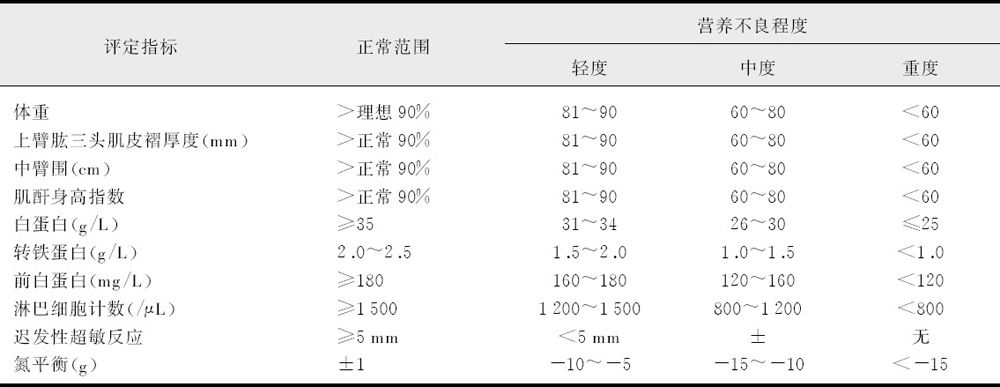
\includegraphics{./images/Image00008.jpg}
\end{table}

\hypertarget{text00003.htmlux5cux23mllj14}{%
\subsection{治疗}\label{text00003.htmlux5cux23mllj14}}

纠治营养不良需采取综合措施,治疗原则为去除病因,调整饮食,补充营养物质,防治并发症,增进食欲,提高消化能力。

(一)去除病因

积极查清病因,治疗消化道疾病、慢性消耗性疾病、感染性疾病等,以去除病因。

(二)合理饮食调整和营养支持

针对病人营养不良程度、消化道能力的强弱以及对食物耐受的情况进行饮食调整,补充足够的营养物质。此时可根据病人的胃肠道功能状况来选择合适的营养补充途径。胃肠道功能良好时,应尽量给予口服膳食调整;如病人不能正常进食而胃肠道功能尚可,应通过管饲喂养;当肠内喂养明显不足或胃肠道功能严重障碍时,则可提供静脉营养支持。

当轻度营养不良病人的消化功能和食物耐受能力均接近正常时,在维持原有膳食的基础上,添加含高蛋白质和高热能的食物。小儿能量供给可从100~120kcal/(kg·d)开始,以后逐渐递增,当供给量达到140~150kcal/(kg·d)时,常获得体重满意的追赶增长,然后再恢复到正常需要量。

当中度和重度营养不良病人的食物耐受能力和全身情况均较差、食欲非常低下甚至丧失时,热能供给要逐渐递增,对重度营养不良病人更要缓慢递增,必要时可提供适量的管饲喂养或静脉营养。通常开始时提供正常需要量的30%~50%,逐渐增加,待一段时间后食欲和消化功能恢复可超过平时生理需要量。食物补充以高蛋白质饮食为主,同时脂肪和碳水化合物的补充也应逐渐保证,以及补充足够的各种维生素和微量元素。在增加过程中,应观察病人胃肠道耐受性和全身症状,勿操之过急。对于严重营养不良的小婴儿,经口喂养的能量供给可自每天40~60kcal/kg开始,根据胃肠道耐受情况可逐渐增加至每天100~140kcal/kg,必要时可再提高至每天150~170kcal/kg,以促进体重增长。如体重增长良好,体重与身高的比例接近正常,能量的供给应再恢复到每天正常生理需要量。

(三)增进食欲,提高抵抗力

可口服胃蛋白酶、胰酶或多酶制剂,以提高食欲和消化能力。口服肠道微生态制剂,有助于促进机体对营养物质的分解和吸收。补充锌元素具有提高味觉的阈值,增加食欲的作用。补充某些激素如生长激素、小剂量胰岛素或蛋白同化类固醇如苯丙酸诺龙等,有促进蛋白质合成、增进食欲的作用。

(四)并发症治疗

{1.贫血}
 贫血是常见的临床症状。轻度贫血可通过饮食治疗,增加含铁丰富的食物摄入,如动物肝脏、动物血和红色肉类等;中度贫血需口服铁剂及维生素C,也可根据体重注射铁剂;严重贫血则需输全血或红细胞。严重水肿型病人除了因贫血而出现虚脱或心力衰竭外,通常不宜输血。

{2.水和电解质紊乱}
 临床上一些病人并非死于饥饿,而是死于治疗时的水和电解质紊乱,轻度和中度紊乱者经饮食及水、电解质补充后即可纠正。严重者则应密切监测病情变化,根据化验结果调整补液量、配方组成和输注速度。

{3.其他}  重视对感染、低血糖、心力衰竭等并发症的监测和对症处理。

\hypertarget{text00003.htmlux5cux23mllj15}{%
\subsection{预防}\label{text00003.htmlux5cux23mllj15}}

营养不良的预防至关重要,预防工作的重点应该是加强营养保健的宣传,进行营养指导,宣传合理的喂养和饮食知识,注意卫生,预防疾病。

(一)营养指导

积极给予营养宣教和膳食指导,重点是《中国居民膳食指南》和平衡膳食宝塔,以及《特定人群膳食指南》的推广。日常饮食中应强调食物成分的正确搭配,对偏食、挑食,以及不良的饮食习惯和习俗予以纠正。对婴幼儿大力鼓励母乳喂养,生后4个月内完全母乳喂养,4~6个月应逐渐按需添加辅食。母乳不足者,或不宜母乳喂养者应采取合理的混合喂养或人工喂养。不应该单独供给淀粉类或炼乳、麦乳精等喂养。接受上述营养教育的对象不仅是病人、家属或普通人群,还包括医务工作者在内的相关职业人员。

(二)补充能量和蛋白质

在人类膳食中能量和蛋白质是首位重要的营养物质,每天都应补足,并注意充分发挥食物蛋白质的互补作用,荤素食物搭配,全面改善营养。

(三)注意卫生,防治疾病

改善个人和环境卫生,防止急、慢性传染病的发生,注意食具的消毒,防止胃肠道疾病的发生,按期进行预防接种,对唇裂、腭裂、先天性肥厚性幽门狭窄进行及时处理。

(四)营养评价表和生长发育监测图的应用

对特殊人群,如住院病人、入住养老和幼托机构的人群应定期接受营养评估或生长发育的监测,如发现存在营养不良或生长落后现象,应及时寻找原因,予以处理。

(五)合理安排生活制度

保证睡眠,适当的户外运动和身体锻炼,使生活具有规律性。

\hypertarget{text00003.htmlux5cux23mllj16}{%
\section{ 维生素缺乏病}\label{text00003.htmlux5cux23mllj16}}

\hypertarget{text00003.htmlux5cux23mllj17}{%
\subsection{维生素A缺乏症}\label{text00003.htmlux5cux23mllj17}}

维生素A族的原形化合物是全反式视黄醇,天然维生素A只存在于动物体内,并分两种类型:维生素A\textsubscript{1}
(视黄醇)和维生素A\textsubscript{2}
(3-脱氢视黄醇)。维生素A是人体必需的微量营养素,对视觉发育、免疫功能、生殖系统、生长发育等均有重要作用,最近研究还发现维生素A参与脑发育。维生素A缺乏症好发于6岁以下婴幼儿,1~4岁为发病高峰。2004年WHO调查结果显示,维生素A缺乏的学龄前儿童有2.5亿,孕妇有2000万。据WHO报道,因维生素A缺乏,全世界每年有50万名学龄前儿童患有活动性角膜溃疡,600万人患干眼症,孕妇患夜盲症高达500万人。原发性维生素A缺乏一般是因膳食中长期匮乏维生素A所引起的。它是以缺少胡萝卜素的大米为主食的南亚和东亚地区的地方性流行病。

(一)发病机制及病因

{1.摄入不足}
 初生时维生素A在肝脏中的贮存量很少,出生后维生素A的主要来源是食物。母乳中的维生素A含量丰富,一般母乳喂养的小儿不会发生维生素A缺乏症,故提倡母乳喂养。早产儿肝脏内维生素A的贮存量更少,且脂肪吸收能力也有限,生长发育的速度又较快,故更容易发生维生素A缺乏症。长期以糕、面糊等谷物或脱脂乳炼乳喂哺小儿而未及时添加辅助食品,或病后“忌嘴”及长期素食都容易发生维生素A缺乏症。如在疾病状态下,长期静脉输液未补充维生素A,也将导致维生素A缺乏。

{2.吸收减少}
 维生素A缺乏可见于多种临床情况,如吸收障碍综合征、慢性腹泻、慢性痢疾、慢性肝炎、胆道梗阻、胆囊纤维化、钩虫病、肠道感染等均可影响维生素A的吸收。长期服用石蜡油通便或某些减肥药(脂肪酶抑制剂如奥利司他)也可影响维生素A的吸收。

{3.锌摄入不足}
 当锌缺乏时,维生素A结合蛋白、前白蛋白、维生素A还原酶都减少,使维生素A不能利用而排出体外,造成维生素A缺乏。Rahman等证实锌的缺乏限制了维生素A的生物利用率,锌和维生素A的缺乏经常同时存在于营养不良的小儿,同时给予维生素A和锌的补充可以改善维生素A的缺乏。近来有报道指出,铁的不足对维生素A的利用也有影响。

{4.消耗增加}
 重体力劳动需要量增加,当供给量不能满足机体需要时,导致维生素A不足;急性或慢性肾炎时,大量蛋白从尿中排出,亦易造成维生素A的丢失,体内维生素A的贮存量减少,造成维生素A的缺乏;各种急、慢性传染病长期发热和肿瘤等均可使机体对维生素A的需要增多,如此时未予及时补充,则造成维生素A的血浆浓度降低。

{5.利用障碍}
 如患有肝脏、肾脏、甲状腺疾病和胰腺囊性纤维变性,以及蛋白质-能量营养不良时,将导致血浆中视黄醇结合蛋白(RBP)代谢异常,导致维生素A缺乏。

(二)临床表现

{1.眼部损害}
 由于维生素A和维生素A原缺乏所引起的营养缺乏病,临床上首先出现暗适应能力下降,最初为暗适应时间延长,以后在暗光下视力减退,黄昏时视物不清,继则发展成夜盲症;眼干燥不适,经常眨眼,系因泪腺管被脱落的上皮细胞堵塞使眼泪减少所致,继而眼结膜和角膜失去光泽和弹性,眼球向两侧转动时可见球结膜折叠形成与角膜同心的皱纹圈,在近角膜旁有泡沫状小白斑,不易擦去,即为毕脱(Bitot)斑;角膜干燥、混浊而软化,继则形成溃疡,易继发感染,愈合后可留下白斑,影响视力;重者可发生角膜穿孔、虹膜脱出而致失明。通常为双侧性的,单侧发病少见。

{2.皮肤病变}
 维生素A缺乏也可引起皮肤的改变,开始时皮肤较正常干燥,以后由于毛囊上皮角化,发生角化过度的毛囊性丘疹,主要分布在大腿前外侧、上臂后侧,后逐渐扩展到上下肢伸侧、肩和下腹部,很少累及胸、背和臀。丘疹坚实而干燥,暗棕色,多为毛囊性,针头大至米粒大,圆锥形。丘疹的中央有棘刺状角质栓,触之坚硬,去除后留下坑状凹陷,无炎症,无主观症状,丘疹密集犹似蟾蜍皮,称为蟾蜍皮病(phrynoderma)。皮疹发生在面部,可有许多黑头。病人毛发干燥、缺少光泽、易脱落、弥漫稀疏;指甲变脆,表面有纵横沟纹或点状凹陷。

{3.生长落后}
 缺乏维生素A的动物最早表现为身高增长缓慢、体重不增、食欲减退。印度学者有研究证明给轻度维生素A缺乏的儿童补充维生素A,结果体重、身高都明显增加。

维生素A缺乏对骨骼生长,特别是对长骨的生长有明显影响,使骨变得又短又厚。亚临床维生素A缺乏可致骨骼发育停止,颅骨和脊柱骨生长受到影响,而且可使骨骼失去正常结构。Hu
W等人通过色层分析法测定维生素A浓度,证明维生素A浓度和体重以及BMI有明显的统计学意义,提示维生素A对儿童的生长发育有明显的影响。

{4.呼吸系统影响}
 维生素A缺乏时,对呼吸系统也有不同程度的影响,使气管及支气管的上皮细胞中间层的细胞增殖,变成鳞状、角化,并使上皮细胞的纤毛脱落,失去上皮组织的正常保护功能,容易发生呼吸系统的感染。

{5.免疫功能受损}
 维生素A可促进细胞分化,有助于维持上皮组织的完整性,在维生素A缺乏症时,不仅仅黏膜屏障作用降低,使得病原体容易入侵,更重要的是局部分泌型IgA水平下降,使得病原体在感染的局部容易繁殖,致病性和炎症作用增强。维生素A缺乏可使机体细胞免疫功能降低,因呼吸道、胃肠道、泌尿生殖道黏膜上皮增生、角化、脱屑,防御功能减弱,容易引起感染。一些研究资料表明,人或动物缺乏维生素A可导致$\text{CD}^+_4$
细胞减少,$\text{CD}^+_4$
/$\text{CD}^+_8$
下降,淋巴细胞增殖,白细胞介素-2(IL-2)、肿瘤坏死因子-α(TNF-α)的分泌减少,T细胞及B细胞增殖减低。人体免疫缺陷病毒(HIV)阳性的母亲血清维生素A水平下降者,其胎儿受HIV传播的发生率可能增加。

(三)实验室检查

{1.视觉暗适应功能测定}
 维生素A缺乏症病人的暗适应能力比正常人差,但其他因素也可引起暗适应能力降低,如视神经萎缩、色素性视网膜炎、睡眠不足等。

{2.血清维生素A水平测定}
 血清维生素A是评价维生素A营养状况的常用指标,也是最可靠的指标,若<0.68μmol/L(200μg/L)为缺乏。正常血清维生素A浓度婴儿为0.68~1.7μmol/L(200~500μg/L),年长儿和成人为1.0~5.1μmol/L(300~1500μg/L)。

{3.血清视黄醇结合蛋白(RBP)测定}
 近来有人认为RBP与人体维生素A水平呈正相关,RBP含量可反映人体维生素A的营养水平。血清视黄醇含量可用免疫测定法或高效液相色谱法直接检测,正常成年人血清视黄醇浓度为1.05~3.15μmol/L,如血清视黄醇浓度在0.35~0.70μmol/L,则表示机体视黄醇含量偏低,肝内视黄醇贮存量不足;WHO
1996年报道:血清视黄醇浓度<0.35μmol/L时,表示视黄醇缺乏,<0.70μmol/L为不足。儿童正常血清视黄醇浓度为>1.05μmol/L,0.70~1.02μmol/L为边缘缺乏,<0.70μmol/L为缺乏。

{4.维生素A的相对剂量反应试验}
 当血清中维生素A浓度在正常范围时,肝脏维生素A已有耗尽的可能,因此采用相对剂量反应(RDR)法间接评价个体体内维生素A的贮存量。测定方法为先测定空腹血清维生素A浓度(A\textsubscript{0}
),随早餐服维生素A450μg,5小时后于午餐前测定血清维生素A浓度(A\textsubscript{5}
)。RDR=(A\textsubscript{5} -A\textsubscript{0} )/A\textsubscript{5}
×100%。若服后5小时的血清维生素A浓度增高幅度,即RDR(relative dose
reation,
RDR)≥20%,表示肝脏内维生素A的贮存已处于临界状态。用此方法可以进一步确定亚临床状态维生素A缺乏。

(四)诊断

仔细询问病史,如病人存在维生素A摄入不足,或存在维生素A的吸收、利用障碍,或引起维生素A消耗过多的疾病,同时合并暗适应障碍、夜盲、结膜干燥、角膜软化,或四肢伸侧有毛囊性角化丘疹,通过暗适应检查和血清维生素A浓度的测定可基本作出诊断。若血清维生素A水平在正常低值,此时肝内维生素A的储存也可能已耗竭。在这种可疑的情况下,可采用敏感而可靠的相对剂量反应试验来进一步确定亚临床维生素A的缺乏。尽量做到早诊断、早治疗,防止严重后果的发生。

(五)治疗

如因为疾病引起维生素A缺乏,应首先去除病因,同时给予维生素A丰富的饮食。用维生素A治疗维生素A缺乏症,疗效迅速而有效。每天补充维生素A2.5万IU(1IU的维生素A=0.3μg的视黄醇),口服或肌注均可,共1~2周(或大剂量1次20万IU),同时给予高蛋白饮食,以后再给予预防量。如有角膜软化则肌注水溶性维生素A10万IU,1周后再给予20万IU,然后给予预防量。夜盲症可于治疗后数小时好转,干眼症于2~3日后改善。必要时保持两眼清洁,使用抗生素眼膏,角膜溃疡者用1%阿托品滴眼防止虹膜粘连。给予维生素A治疗时,同时补充维生素E,可提高疗效。

(六)预防

无论何种类型的维生素A缺乏,只要早期发现,及时治疗,其预后都良好。

{1.供给含维生素A丰富的食物}
 维生素A最好来源是动物性食品,如黄油、蛋类、肝脏、鱼类、肉类、禽类、奶类及其制品,深绿色蔬菜、胡萝卜、番茄等食物为富含胡萝卜素的食品。养成不偏食、不挑食的习惯。维生素A安全摄入量范围较小,大量摄入可引起中毒。

{2.易感人群的维生素A营养状况的监测}
 对婴幼儿、儿童、孕妇、乳母等易感人群进行暗适应能力、眼部症状、血清视黄醇水平等方面的检测,及时发现亚临床缺乏者。

{3.对易感人群进行干预}
 婴幼儿是维生素A缺乏的易感人群,WHO在维生素A缺乏病高发的发展中国家,推广1次口服维生素A20万IU,6~8个月再重复1次,结果证实服药组小儿干眼病和呼吸道、胃肠道疾病的发病率及死亡率均较不服药组明显降低。建议定期补充维生素A制剂是快速改善维生素A状况的方法。对于维生素A严重缺乏地区,WHO和UNCEF推荐:<6个月婴儿一次性补充维生素A5万IU,6~12个月婴儿每4~6个月口服维生素A10万IU,>12个月婴幼儿每4~6个月口服维生素A20万IU,分娩后8周内的孕妇口服维生素A20万IU。

{4.选用维生素A强化食品}
 这是一种防治维生素A缺乏症最直接有效的方法。作为维生素A载体的食物有很多,如糖、味精、大米、面粉、饼干、食用油等。近年来菲律宾在维生素A强化食品方面进行了很多研究,卓有成效。

{5.开展健康教育}
 可通过社区、家庭及学校开展教育,养成良好的饮食习惯,提高人群自我保健意识。

\begin{center}\rule{0.5\linewidth}{\linethickness}\end{center}

[附]

维生素A过多症

维生素A过多症(hypervitaminosis
A),即维生素A中毒,根据发病情况,可分为急性中毒及慢性中毒两种。当血清维生素A浓度超过5.1μmol/L(1500IU/L)时可出现中毒症状。过去曾报道过极区探险者因大量食用维生素A含量丰富的北极熊肝而发生急性中毒。

\textbf{【急性中毒】}
 比较多见,由于短期内大量摄入维生素A所致。成人一次性应用维生素A>30万~100万IU(90~300mg
RE),一次或多次连续摄入膳食推荐摄入量(RNI)的100倍;儿童一次>30万IU(90mg
RE)或多次连续摄入膳食推荐摄入量(RNI)的20倍可致急性中毒。常表现为颅内压增高症状,如烦躁、恶心、呕吐、嗜睡、食欲减退、复视、视神经乳头水肿,囟门未闭者则囟门饱满。

\textbf{【慢性中毒】}
 慢性中毒是服用维生素A20~30倍于推荐剂量(RDA),或长期较大剂量摄取维生素A所致。成人每天摄入8万~10万IU(24~30mg
RE)持续半年或每天3万~4万IU(9~12mg
RE)超过8年,婴儿每天摄入5万~10万IU(15~30mg
RE)超过6个月可致慢性中毒。常发生在因慢性皮肤疾病服药的病人。一般摄入数周或数月后出现症状,表现为慢性症状,如食欲减退、嗜睡、不适,有时伴有腹部不适,骨或关节疼痛严重时有搏动性头痛、失眠、烦躁不安、体毛脱落和指甲变脆。有时还发生便秘、月经不规则、情绪不稳等。幼儿期有服用大量维生素A引起的维生素A过多症,主要表现为肝脾肿大、红细胞和白细胞减少、骨骼症状(有骨痛,以长骨为主),骨骼X线表现为骨皮质增厚、骨膜下积液和骨膜分离,以骨中段更明显。

\textbf{【处理】}
 一旦发现维生素A过多,应立即停服维生素A制剂及对症处理。急性中毒者,待停服维生素A,1~2天后症状缓解;慢性中毒者,待停服维生素A1~2周后症状减轻或消失,但骨骼X线表现需要半年左右恢复正常。

\begin{center}\rule{0.5\linewidth}{\linethickness}\end{center}

\hypertarget{text00003.htmlux5cux23mllj18}{%
\subsection{维生素D缺乏病}\label{text00003.htmlux5cux23mllj18}}

维生素D是维持高等动物生命所必需的营养素,它是钙代谢最重要的生物调节因子之一。维生素D不足将导致维生素D缺乏(vitamin
D
deficiency)性佝偻病,这是一种慢性营养缺乏病,主要见于3岁以下婴幼儿。老人由于生活习惯改变、生理代谢功能减退,饮食营养状况也发生变化,维生素D缺乏病同样不能忽视。婴幼儿时期出现维生素D缺乏则可导致佝偻病的发生,成人阶段的维生素D缺乏则形成骨软化症。与骨软化症相比,佝偻病具有很高的发生率。17世纪,Francis
Glisson教授和Daniel
Whistle医生首先科学地描述了维生素D缺乏症,即佝偻病。此病是以维生素D缺乏导致的钙、磷代谢紊乱和骨骼的钙化障碍为主要特征。佝偻病发病缓慢,不容易引起家长的重视。佝偻病使小儿抵抗力降低,容易合并肺炎及腹泻等疾病,影响小儿生长发育。因此,必须积极防治。

(一)体内来源及代谢特征

人体内的维生素D可从两个途径,即经皮肤内转化形成和经口摄入获得,前者称内源性维生素D,后者称外源性维生素D。内源性维生素D是人体皮肤内的7-脱氢胆固醇经日光中的紫外线照射后产生没有活性的维生素D\textsubscript{3}
;外源性维生素D来自食物,如鱼、肝、蛋、乳类等含有较丰富的维生素D\textsubscript{3}
。膳食中的维生素D\textsubscript{3}
在胆汁的协助下,在小肠内形成乳糜微粒被吸收入血浆,与内源性维生素D\textsubscript{3}
一起经维生素D\textsubscript{3}
结合蛋白(血浆内的一种α-球蛋白)转运至肝脏。在肝内经25-羟化酶的催化作用下氧化成为25-(OH)\textsubscript{2}
D\textsubscript{3}
,此时,虽已具有抗佝偻病活性,但作用不强,再被转运至肾脏后,经1-羟化酶的催化进一步被氧化成具有较强抗佝偻病活性的1,25-(OH)\textsubscript{2}
D\textsubscript{3} ,最后经血循环输送到相关靶器官而发挥其生理作用。

转运至小肠组织的1,25-(OH)\textsubscript{2} D\textsubscript{3}
先进入肠黏膜上皮细胞内,与胞质中的特异性受体形成复合体,作用于核内染色质,诱发合成特异的钙结合蛋白,后者的作用是把肠腔表面的钙离子转运带入黏膜细胞,从而进入血液循环使血钙升高,促进骨中钙的沉积。除此以外,1,25-(OH)\textsubscript{2}
D\textsubscript{3}
对肾脏也具有直接作用,它促进肾小管对钙和磷的重吸收,以减少钙和磷的丢失。

(二)病因

{1.日光照射不足}
 日光照射下皮肤内维生素D的合成是体内维生素D的主要来源。如日照不足,尤其在冬季,需定期通过膳食补充。此外,空气污染也可阻碍日光中的紫外线,人们日常所穿的衣服、住在高楼林立的市区、生活在室内、使用人工合成的太阳屏障等阻碍紫外线、居住在日光不足地区等都可影响皮肤生物合成足够量的维生素D。资料显示,在纬度较高的北方地区,居民血浆25-(OH)\textsubscript{2}
D\textsubscript{3}
的含量存在明显的季节波动。日光浴是使机体合成维生素D\textsubscript{3}
的重要途径之一。

{2.维生素D和钙、磷摄入不足}
 动物性食品是天然维生素D的主要来源,海水鱼如鲱鱼、沙丁鱼,动物肝脏,鱼肝油等都是维生素D\textsubscript{3}
的良好来源。尽管从普通的食物如鸡蛋、牛肉、黄油和植物油中也可获得少量的维生素D\textsubscript{3}
,但日常一般膳食中所含的维生素D是不能满足机体需要的。因此,对于日光暴露不理想的人群,尤其在冬季,维生素D的补充特别显得重要。2岁以内的婴幼儿,由于暴露阳光不充足,乳类又含维生素D不足,且处于快速生长阶段,容易造成体内维生素D的缺乏。因此建议多晒太阳,同时补充鱼肝油。

另外,食物中钙、磷含量不足以及比例不当均可影响钙、磷的吸收。人乳中钙、磷含量虽低,但比例(2∶1)适宜,容易被吸收;而牛乳钙、磷含量较高,但钙磷比例(1.2∶1)不是最佳比例,故牛乳中的钙吸收率没有人奶高。

{3.钙、磷、维生素D需要量增多}
 早产儿因生长速度快和体内储钙不足而易患佝偻病;婴儿生长发育快,对维生素D和钙的需要量增多,故易引起佝偻病;2岁后因生长速度减慢,且户外活动增多,佝偻病的发病率逐渐减少。

{4.疾病影响}
 肝、肾疾病及胃肠道疾病影响维生素D、钙、磷的吸收和利用。小儿胆汁郁积、总胆管扩张、先天性胆道狭窄或闭锁、脂肪泻、胰腺炎、难治性腹泻等疾病均可影响维生素D、钙、磷的吸收而患佝偻病。

{5.药物影响}
 长期使用苯妥英钠、苯巴比妥(鲁米那)等药物,可加速维生素D的分解和代谢而引起佝偻病。

(三)发病机制

维生素D缺乏时,1,25-(OH)\textsubscript{2} D\textsubscript{3}
生成减少,钙、磷经肠道吸收减少,使血钙降低刺激甲状旁腺激素(parathyroid
hormon,
PTH)分泌增多。PTH能诱导破骨细胞生成,从而对骨质进行溶解和吸收,临床上出现骨样组织钙化障碍的表现;同时成骨细胞代偿性增生,局部骨样组织堆积,碱性磷酸酶分泌增多,临床上同样产生一系列相应的骨骼改变和生化改变。另外,PTH又反馈促进肾脏形成1,25-(OH)\textsubscript{2}
D\textsubscript{3}
,从而增加小肠和肾小管对钙的吸收,而PTH抑制肾小管对磷的重吸收,此时尿磷大量排出,尿钙则趋于正常或稍偏低,故当维生素D缺乏时临床常发生低磷血症。

(四)病理改变

维生素D缺乏引起钙、磷代谢紊乱,导致骨样组织钙化不良、骨骼生长障碍。在骨骺尚未联合前的儿童期发病称为佝偻病;在骨骺板已闭的成人则发生骨钙化障碍,导致骨软化病。佝偻病的主要病理改变是骨样组织增生,骨基质钙化不良。维生素D缺乏时,钙、磷沉积于骨受阻,成骨作用发生障碍,长骨干骺端的骨骺软骨中成熟软骨细胞及成骨细胞不能钙化而继续增殖,形成骨骺端骨样组织堆积,临时钙化带增厚,骨骺膨大,形成临床上常见的肋骨串珠、手镯、脚镯征等,使骨的生长发育停滞不前。长骨骨干因骨质脱钙,骨皮质被不坚硬的骨样组织代替,故骨干容易弯曲畸形,甚至发生病理性骨折。颅骨骨化障碍表现为颅骨软化,颅骨骨样组织堆积造成方颅和骨骼畸形。

(五)临床表现

维生素D缺乏性佝偻病是婴幼儿中常见的营养缺乏症,多发生于3个月~2岁的小儿,主要为骨骼的改变,肌肉松弛,以及非特异性的精神神经症状。重症佝偻病病人可影响消化系统、呼吸系统、循环系统及免疫系统功能,同时对小儿的智力发育也有影响。

维生素D缺乏性佝偻病在临床上分为初期、激期、恢复期和后遗症期。初期和激期统称为活动期。

{1.初期}
 多数从3个月左右开始发病,此期以精神神经症状为主,患儿有睡眠不安、好哭、易出汗等现象,出汗后头皮痒而在枕头上摇头摩擦,出现枕部秃发。

{2.激期}
 除初期症状外,患儿以骨骼改变和运动功能发育迟缓为主。用手指按在3~6个月患儿的枕骨及顶骨部位,感觉颅骨内陷,随手放松而弹回,称乒乓球征。8~9个月以上的患儿头颅常呈方形,前囟大及闭合延迟,严重者18个月时前囟尚未闭合。两侧肋骨与肋软骨交界处膨大如珠子,称肋串珠。胸骨中部向前突出形似“鸡胸”,或下陷成“漏斗胸”,胸廓下缘向外翻起为“肋缘外翻”。会站、走的小儿由于体重压在不稳固的二下肢长骨上,两腿会形成向内或向外弯曲畸形,即“O”型或“X”型腿。

患儿的肌肉韧带松弛无力,因腹部肌肉软弱而使腹部膨大,平卧时呈“蛙状腹”,因四肢肌肉无力,学会坐、站、走的年龄都较晚,因两腿无力容易跌跤。出牙较迟,牙齿不整齐,容易发生龋齿。大脑皮质功能异常,条件反射形成缓慢,患儿表情淡漠,语言发育迟缓,免疫力低下,易并发感染、贫血。

{3.恢复期}
 经过一定的治疗后,各种临床表现均消失,肌张力恢复,血液生化改变和X线表现也恢复正常。

{4.后遗症期}
 多见于3岁以上小儿,经治疗或自然恢复后临床症状消失,仅重度佝偻病遗留不同部位、不同程度的骨骼畸形。

以上各期的血液生化学与X线检查结果见表2-4。

\begin{table}[htbp]
\centering
\caption{维生素D缺乏性佝偻病各期的血液生化学检查及X线检查}
\label{tab2-4}
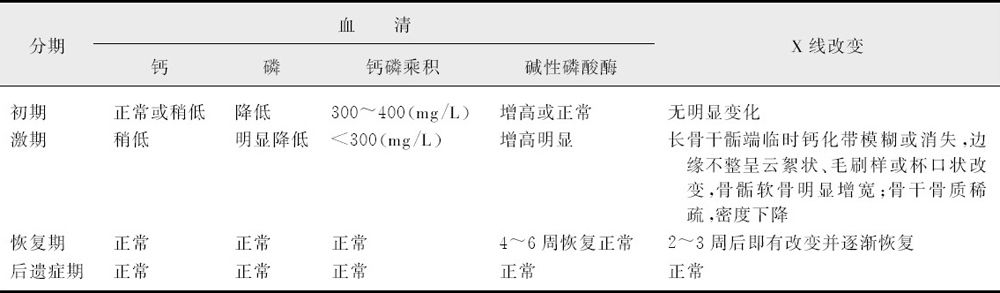
\includegraphics{./images/Image00011.jpg}
\end{table}

(六)诊断

根据病史、症状、体征及血液生化学检查及骨X线检查的改变可作出诊断。对可疑病例应测定血钙、磷、碱性磷酸酶,同时行骨龄X线摄片检查,血清25-(OH)\textsubscript{2}
D\textsubscript{3} 和1,25-(OH)\textsubscript{2} D\textsubscript{3}
在佝偻病活动早期就明显降低,血浆中cAMP浓度和尿的排泄量均增高,尿钙的测定也有助于佝偻病的诊断。

(七)治疗

{1.一般治疗}
 哺乳期婴儿要强调补充鱼肝油,及时添加含维生素D较多的食品(肝、蛋黄等),多到户外活动,增加日光直接照射的机会。激期阶段勿使患儿久坐、久站,防止骨骼畸形。

{2.补充维生素D}
 初期每天口服维生素D125~250μg(5000~10000IU),持续1个月后改为预防量。激期250~500μg(10000~20000IU)口服,连服1个月后改为预防量。维生素D大剂量突击疗法:初期肌注维生素D\textsubscript{3}
7500μg(30万IU),一般注射1次即可,同时停服维生素D制剂,1个月后改预防量口服。激期肌注维生素D\textsubscript{3}
7500μg(30万IU),根据病情,1个月后可重复注射1次,再隔1个月改为口服预防量。

{3.补充钙剂}  维生素D治疗期间应同时服用钙剂。

{4.矫形疗法}
 轻度骨骼畸形在治疗后或在生长过程中自行矫正。应加强体格锻炼,可做些主动或被动运动的方法矫正。例如,俯卧撑或扩胸动作使胸部扩张,纠正轻度鸡胸及肋外翻。严重者,4岁后可考虑手术矫行。

(八)预防

最好的预防是晒太阳。人体所需维生素D约80%靠自身合成,有人测定,阳光直晒后,每平方厘米皮肤在3小时内能合成维生素D18IU。据报道,婴儿预防佝偻病所需日光浴的时间为每周30分钟,穿衣不戴帽为每周120分钟。春夏季出生的孩子满月后就可抱出户外,秋冬季出生的孩子3个月也可抱出户外,开始每次外出逗留10~15分钟,以后可适当延长时间,如在室内应开窗。

正确喂养对预防也有重要意义,母乳喂养的婴儿自出生后1周开始每天补充维生素D400IU,早产儿每天补充800IU。及时添加辅食,断奶后要培养良好的饮食习惯,不挑食、不偏食,保证小儿各种营养素的需要。对早产儿、双胎儿、人工喂养儿,应用维生素D预防仍是重要方法。

\begin{center}\rule{0.5\linewidth}{\linethickness}\end{center}

[附]

维生素D过多症

长期大量服用或短期超量误服维生素D或对维生素D过于敏感,均可引起维生素D过多症(hypervitaminosis
D),临床上出现以高钙血症引起的临床中毒症群。中毒剂量个体差异很大,与维生素D的剂量、应用时间和给药途径有关。通常每天摄入维生素D3000~8000IU 1~3个月可出现中毒症状。

\textbf{【临床表现】}
 主要系因血钙过高和钙盐沉积于身体各组织器官所致。最早症状为厌食,继之出现体重减轻、低热、精神不振、恶心、呕吐、顽固性便秘、嗜睡、表情淡漠,年长儿诉头痛,重者或晚期可出现高热、多尿、烦躁、脱水、昏迷、抽搐等症状。严重者可因高钙血症导致主动脉瓣钙化及狭窄、肾钙化及肾功能衰竭而致死。

\textbf{【实验室检查】}
 血钙增高(>3.0mmol/L),尿钙增加,尿蛋白阳性,血尿素氮增高。X线长骨摄片,临时钙化带过度钙化、密度增高,骨皮质增厚,骨小梁密度增高而模糊,其他组织器官可出现异位钙化灶。

\textbf{【处理】}
 立即停用维生素D,处理高钙血症,限制钙盐摄入,给利尿剂加速钙的排泄,同时应用泼尼松或氢氧化铝抑制肠道对钙的吸收。亦可试用合成降钙素50~100IU/d,皮下或肌注。注意水及电解质平衡。

\textbf{【预防】}
 加强宣传,使家长了解维生素D并非滋补药,应掌握用量及时间。

\begin{center}\rule{0.5\linewidth}{\linethickness}\end{center}

\hypertarget{text00003.htmlux5cux23mllj19}{%
\subsection{维生素K缺乏症}\label{text00003.htmlux5cux23mllj19}}

维生素K分为两大类:一类是脂溶性维生素,即K\textsubscript{1}
(从植物中提取)和K\textsubscript{2}
(从微生物中提取,也可由肠内细菌合成);另一类是水溶性维生素,即K\textsubscript{3}
和K\textsubscript{4} (由人工合成),其中以K\textsubscript{1}
和K\textsubscript{2}
最为重要。维生素K是促进血液凝固的化学物质之一,是4种凝血蛋白(凝血酶原、转变加速因子、抗血友病因子和司徒因子)在肝内合成必不可少的物质。维生素K的缺乏将导致凝血功能失常,而出现出血。维生素K缺乏症(vitamin
K
deficiency)是由于维生素K缺乏引起的凝血障碍性疾病。本病常见于3个月内单纯母乳喂养而母亲不吃蔬菜的小儿,尤以新生儿期出血为多见。婴儿期小儿亦不少见。

(一)病因

本病的发病原因是由于体内维生素K缺乏,使凝血因子Ⅱ、Ⅶ、Ⅸ、Ⅹ在肝内合成不足,从而引起出血。根据发病的早晚分成以下3种类型。

{1.早发型}
 多见于新生儿出生后24小时内发病。在婴儿出生后1小时内即可出现,常导致致命性出血。发病原因有以下2种。

(1)母体缺乏维生素K,维生素K经胎盘转运不足,经放射免疫方法检测大部分新生儿脐血中维生素K缺乏。

(2)孕期药物影响:母亲怀孕期间服用影响维生素K代谢及合成的药物能导致新生儿期维生素K缺乏。如果长期应用抑制肠道内细菌生长的药物,如广谱抗生素和肠道内不易吸收的磺胺类药物,能抑制肠道内寄生的非致病菌,减少肠道内维生素K的合成,导致维生素K的缺乏。口服抗凝药物如双香豆素的结构与维生素K相似,可与维生素K竞争,减少凝血酶原在肝脏内的合成:孕妇服用抗惊厥药物后,可经胎盘输送,并以类似抗凝药物的作用来抑制维生素K的生成,引起新生儿维生素K的缺乏。摄入过量的维生素A,也能抑制维生素K\textsubscript{2}
的肠内合成,并且因为维生素K\textsubscript{1} 、K\textsubscript{2}
均为脂溶性物质,其他脂溶性维生素如维生素A和维生素D都能影响其吸收。

{2.经典型}  生后2~3天发病,早产儿可迟2周。其原因为以下3种。

(1)单纯母乳喂养:母乳喂养是婴儿最佳的喂养方式已得到公认,应该大力提倡和推广,但由于人乳中含维生素K的量极低,初乳中几乎不含维生素K,人乳中维生素K含量平均为15μg/L(牛奶中含量为60μg/L)。另外,母乳含有多种抗体,这些抗体有利于抵抗婴儿肠道和呼吸道的感染,但同时也抑制了肠道内能合成维生素K的细菌如脆弱杆菌和某些大肠埃希菌的生长。如单纯母乳喂养的婴儿未给予适当量的维生素K补充,很容易导致维生素K缺乏。据相关文献报道,90%以上的维生素K缺乏性出血是发生在母乳喂养的婴儿中。

(2)吸收利用功能不良:新生儿,特别是早产儿胆汁分泌有限,且胆汁中胆酸含量少,脂肪及脂溶性维生素吸收不良,影响维生素K的吸收。这在患有肝胆系统疾病的婴儿,如先天性胆道闭锁、胆总管囊肿和胆汁淤积等时更常见。再者新生儿及早产儿肝脏功能未发育成熟,使凝血因子Ⅱ、Ⅶ、Ⅸ、Ⅹ在肝内合成不足,以致维生素K依赖因子生成减少。

(3)体内合成减少:新生儿出生时肠道内几乎无细菌,维生素K合成不足。

{3.迟发型}  多发生于出生后1个月。发病原因有以下4种。

(1)摄入不足:新生儿摄奶量少且母乳中维生素K含量低,如长期单纯母乳喂养,未及时添加辅食,未添加含维生素K丰富的蔬菜、水果,均可引起维生素K缺乏。

(2)吸收不良:因慢性腹泻、溃疡性结肠炎、肠切除、囊性纤维化等疾病引起的小儿肠道吸收不良,均可引起维生素K吸收障碍,以及胆道阻塞、胆瘘等胆道梗阻性或胆汁缺乏性疾病,均可影响维生素K的吸收。

(3)利用障碍:新生儿肝炎、新生儿败血症及病毒感染等任何原因引起的肝脏损害均可影响维生素K依赖因子的合成。

(4)合成减少:肠道细菌也可合成部分维生素K,在婴儿于肠道菌落出现后,维生素K缺乏情况则明显减少,长期应用抗生素会抑制肠道内正常细菌的生长,也会使维生素K合成减少。

(二)临床表现

临床上以出血为主要表现。早发型者可有头颅血肿,颅内、胸腔内出血。经典型者往往首发症状是脐带出血及胃肠道出血。不能用脐带结扎不良来解释的脐部出血的轻者为渗血,重者则出血不止。胃肠道出血则表现为不同程度吐血和便血。皮肤出血多见于分娩时挤压处,轻者为瘀点和紫癜,重者可形成大片瘀斑和血肿;也可见于采血及注射部位、术后伤口处渗血不止。颅内出血较少见,但早产儿由于毛细血管脆性增加,一旦颅内出血,往往预后不良。迟发型者约90%以上见于单纯母乳喂养儿,单纯母乳喂养儿维生素K缺乏性出血的机会是人工喂养儿的15~20倍,如合并腹泻、使用抗生素、肝胆疾病,以及长期禁食患儿更易发生,常见急性或亚急性颅内出血,以蛛网膜下隙、硬膜下、硬膜外出血为多见,脑室、脑实质出血少见,临床上有严重的中枢神经系统功能异常及颅内高压的表现,表现为高声尖叫、频繁呕吐、反复抽搐,严重的患儿可出现昏迷。同时可伴有出血性贫血。

(三)实验室检查

实验室主要通过检测凝血因子及活性来间接反映维生素K的缺乏。凝血酶原检测是维生素K缺乏的可靠证据。凝血酶原时间(PT)延长多数超过正常对照的2倍,轻度维生素K缺乏仅发现凝血酶原时间延长,而无临床出血倾向。有的维生素K缺乏病人部分凝血活酶时间(KPTT)延长和凝血因子Ⅱ、Ⅶ、Ⅸ、Ⅹ因子活性明显降低。通常第Ⅶ因子首先降至最低,第Ⅶ因子减低后凝血酶原水平随即下降,但较缓慢,第Ⅸ、Ⅹ因子也有不同程度地减少。必要时可行维生素K的浓度及维生素K缺乏诱导蛋白(PIVKA-Ⅱ)的检测。

如疑有颅内出血者应进行B超、CT或MRI检查,以了解出血情况。

(四)诊断

根据病史、症状、体征及临床表现、辅助检查可作出诊断。

{1.详细询问病史}
 了解患儿的喂养情况及辅食添加情况。多见于单纯母乳喂养儿,出生后3个月内的婴儿,未接受过维生素K的预防。

{2.观察病情}
 新生儿出血症多见于出生后1~7天,以胃肠道出血为多见,病情较轻,凝血酶原时间延长,血小板、出血时间均正常,给予维生素K治疗效果良好,数小时或24小时后出血倾向明显好转。迟发性维生素K缺乏性出血症,大多表现为颅内出血、烦躁不安、脑性尖叫、拒奶、嗜睡,体检发现前囟饱满,颅缝增宽,Moro反射、觅食反射消失,但如不伴有其他部位出血的患儿,易误诊为颅内感染,而迟发性出血症表现为突然起病,无明显感染中毒症状,贫血发展迅速而严重,故可与颅内感染相鉴别。

{3.实验室检查}
 PT、KPTT延长,PIVKA-Ⅱ阳性,血清维生素K浓度低下或测不到,血小板和出血时间正常。当颅内出血时,脑脊液检查呈现均匀一致的血性和皱缩红细胞,但脑脊液检查正常也不一定完全排除此病,且病情危重者不宜进行该项检查。

{4.其他}
 有助于诊断的辅助检查有B超、CT及MRI检查,不仅可确定出血部位、范围,还可随访疗效,进行预后判断。给予补充维生素K制剂后出血得到控制。

(五)治疗

有出血现象时,应立即注射维生素K2mg,可迅速改善出血,胃肠道出血者应暂禁食,给予静脉营养支持,根据失血情况适当纠正贫血,严重者可输全血或血浆10~20ml/kg。如有颅内出血,首先要加强护理,保持安静,维持气道通畅,抬高头、肩部,延迟喂奶,适当控制补液;如有高声尖叫、频繁呕吐、反复抽搐等表现,应对症止惊,降低颅内压,恢复脑细胞功能;严重者可手术清除血肿。

(六)预防

预防新生儿维生素K缺乏症应从孕期开始,分娩前数周即可口服维生素K20mg,可预防新生儿维生素K缺乏所致的低凝血酶原血症。乳母应多吃蔬菜、水果以提高乳汁中维生素K含量。

自从1961年美国儿科学会营养委员会提出所有新生儿应在出生后肌注维生素K\textsubscript{1}
0.5~1mg作为预防新生儿出血以来,维生素K\textsubscript{1}
用来预防和根治新生儿维生素K缺乏性出血已在许多国家得到广泛应用。荷兰Cornelissen
EA等实验证明,在新生儿出生后3个月内,每周口服维生素K1mg可有效纠正维生素K缺乏且不会引起维生素K在体内的积聚。加拿大儿科协会建议足月产的新生儿应在出生后6小时内口服或肌注维生素K1mg;早产儿、低体重儿及难产儿均需在产后6小时内肌注维生素K1mg;因脂肪吸收不良而有迟发性出血性疾病危险性的新生儿需每天口服维生素K1mg或每月肌注维生素K1次以预防维生素K缺乏性出血症。我国林良明等于2002年报道中国7省协作对19751例活产婴儿进行对照研究发现,采用给婴儿出生后口服维生素K\textsubscript{1}
2mg,以后每隔10天1次,服满3个月,共10次,对预防维生素K缺乏性出血有相当好的效果。


\subsection{维生素B\textsubscript{1}缺乏症}

维生素B\textsubscript{1}
又称硫胺素,是抗脚气病因子或抗神经炎因子,它是最早发现的维生素之一。维生素B\textsubscript{1}
在高温,特别是高温碱性溶液中易被破坏,在酸性溶液中,稳定性较好。在体内80%维生素B\textsubscript{1}
是以硫胺素焦磷酸盐(TPP)的形式存在,10%是以硫胺素三磷酸盐的形式存在,其余的为硫胺素单磷酸盐或游离的硫胺素。维生素B\textsubscript{1}
缺乏将引起一种典型的疾病,被称为脚气病。早在公元前2600年,古人已对本病作过描述。第一个记录脚气病的是1592年荷兰医生Jacob
Bontius。1897年荷兰医生Eijkman以小鸡做实验,发现用精白米饲养小鸡,即出现一种类似脚气病的多发性神经炎,如用粗米饲养小鸡,则能预防这种疾病。同期Eijkman的朋友Vorderman发现吃自制粗磨大米的犯人的脚气病比吃商品精米的犯人少。1911年,Funk和Suzuki等从稻米碾磨物种分离出一种具有生物活性的结晶化合物。1936年,Williams公布了维生素B\textsubscript{1}
的化学结构,它是由含硫噻唑环联结氨基吡啶环组成,并开始人工合成。

(一)病因

{1.摄入不足}  维生素B\textsubscript{1}
广泛存在于自然界的植物和动物体内。谷类食物是我国大多数居民的维生素B\textsubscript{1}
来源。长期吃精细粮食、膳食制作过程中的丢失(过度碾磨和淘洗),如长期使用精白米、面,以及以淀粉为主食,或煮饭时为增加其黏稠度,而加入少量的碱,将破坏维生素B\textsubscript{1}
,可致摄入量不足。通常母乳中的维生素B\textsubscript{1}
含量能满足婴儿生长需要,但如果乳母膳食中维生素B\textsubscript{1}
的摄入量缺乏,则会引起母乳中的维生素B\textsubscript{1}
不足,如不及时补充也将引起婴儿的维生素B\textsubscript{1} 缺乏症。

{2.吸收不良和利用障碍}
 如患有消化系统疾病,如慢性腹泻、慢性痢疾、胆囊纤维化、肠道感染等疾病,均可减少维生素B\textsubscript{1}
的吸收。肝、肾疾病将影响TPP的合成,造成维生素B\textsubscript{1}
缺乏。维生素B\textsubscript{1}
缺乏使胃液中酸度降低,继而胃肠道中硫胺素复合物内的硫胺素释放也减少,影响了硫胺素的吸收。

{3.需要量增加或消耗过多}
 长期患有消耗性疾病,如甲状腺功能亢进、结核或长期发热等,糖尿病、尿崩症等尿量排出多时使维生素B\textsubscript{1}
的丢失增加,高温作业、重体力劳动、小儿于快速生长发育期及妊娠期等需要量也相对增多。如未予及时补充,则易造成维生素B\textsubscript{1}
的缺乏。

{4.遗传代谢障碍}  遗传性维生素B\textsubscript{1}
代谢与功能障碍,引起的维生素B\textsubscript{1}
缺乏症,一般具有高度的家族性遗传性疾病史,或父母近亲结婚史。

(二)病理生理

机体中TPP是丙酮酸氧化脱羧酶系的辅助因子,是丙酮酸进入三羧酸循环氧化放能的重要辅酶;也是磷酸己糖氧化支路中转羧乙醛酶的辅酶。因此维生素B\textsubscript{1}
与糖代谢密切相关,其缺乏使糖代谢受阻,能量产生减少,结果使神经组织、骨骼肌和心肌缺乏主要的能量来源,血液和组织内丙酮酸及乳酸堆积,产生一系列的病理变化。

{1.神经系统}
 尤其是末梢神经受损严重,髓鞘退化及色素沉着,雪旺(Schwann)细胞呈空泡变性。中枢神经系统和周围神经系统的神经纤维的髓鞘发育不良,因此表现为易激惹。重者神经轴被破坏,出现断裂萎缩,以坐骨神经及其分支受累较为常见,并且临床症状出现较早。其他如前臂神经等亦可累及。

{2.心血管系统}
 由于能量缺乏,导致心肌水肿、纤维粗硬、心肌无力,严重时发生心力衰竭。心脏扩张肥厚,尤以右心室明显,血管充血,但组织结构正常。周围血管平滑肌张力下降、小血管扩张。

{3.组织水肿及浆膜腔积液}
 组织水肿多见于下肢,当体腔浆液渗出时,可见心包腔、胸腔及腹腔积液。

{4.肌肉萎缩}
 出现于受累神经支配的肌肉。镜下可见肌纤维横纹消失、混浊肿胀及脂肪变性。

{5.消化系统}  消化道平滑肌张力下降,影响胃肠蠕动,消化功能减弱。

(三)临床表现

维生素B\textsubscript{1}
缺乏将导致脚气病。脚气病是维生素B\textsubscript{1}
摄入不足的最终结果。本病主要影响心血管和神经系统,主要表现为多发性神经炎、肌肉萎缩、组织水肿、心脏扩大、循环失调及胃肠症状。临床表现可因发病年龄及受累系统不同而异。婴幼儿起病较急,成人起病则较缓。一般可分为亚临床型、神经型(干型和脑型脚气)和心血管型(湿型脚气)和婴儿脚气病。

{1.亚临床型}  多见于维生素B\textsubscript{1}
供给量不能满足机体需要,且持续3个月以上的病人。病人常感疲乏无力、烦躁不安、易激动、头痛、食欲不振、下肢倦怠、酸痛。如病情进一步发展则出现典型的神经和(或)心血管型表现。

{2.神经型}
 ①周围神经系统累及较为常见。主要发生在远端肢体,下肢发病较上肢早,且感觉异常先于运动障碍,先远端后近端,呈对称性。初时,病人感觉下肢软倦、无力,有针刺或烧灼感等过敏症状,肌肉酸痛以腓肠肌最为明显,有时出现腓肠肌抽搐、痉挛,甚至不能行走。随着病情发展出现肢体麻痹,呈手套或袜子样感觉障碍。进一步发展出现肢体肌肉萎缩,如伸肌受累可发生足下垂和(或)腕下垂;如累及喉返神经则出现声音嘶哑。②中枢神经系统受累称脑型脚气病综合征(Wernicke脑病),一般人群较罕见,常见于酗酒病人。临床上一般按以下顺序发展:呕吐、眼球震颤、眼肌麻痹、跨越步态和共济失调、进行性精神衰退以至精神异常,最后可发生昏迷及死亡。

{3.心血管型}
 病程可呈慢性经过,逐渐出现心悸、气促、心前区胀闷;心尖区可闻及收缩期杂音及第三心音;舒张压降低,脉压差增宽,可有水冲脉和毛细血管搏动。X线检查显示心脏扩大,肺动脉弓突出和右心扩大为其特征。心电图表现为低电压、P-R间期缩短、Q-T时间延长,T波平坦、双相或倒置。病情发展可因循环衰竭而死亡。另外,水肿为湿型脚气病人的常见症状,起初从足踝部开始,继而发展至小腿、膝和整个下肢甚至全身,严重时可有胸腔、心包腔和腹腔等处积液,并可迅速发展至循环衰竭而死亡。

{4.婴儿型脚气病}
 多发生于数个月的婴儿,发病急、突然,较成人型难以捉摸,可出现多种临床表现,发病初期主要表现为消化系统症状,如食欲不振、厌食、恶心、呕吐、腹痛、便秘或腹泻,不久就出现神经系统症状,可分为脑型或神经炎型。脑型表现主要为发作型哭叫似腹痛状,烦躁不安,前囟饱满,头后仰;严重者可发生脑充血、颅内高压、昏迷而死亡。神经炎型主要表现为周围性瘫痪,早期表现为四肢无力,其后,症状加重,同时足趾的背屈运动受限。跟腱反射和膝反射初期增强,随后减弱,最后消失。软腭反射障碍,吃奶出现呛咳,吞咽困难。心血管主要表现为心动过速,婴儿可出现奔马律、呼吸困难,晚期出现紫绀、心脏扩大、心力衰竭、肺充血及肝淤血。水肿可遍及全身,多发生于下肢,浆膜腔积液也可发生于心包腔、胸腔和腹腔。由于喉的水肿而出现失声,或出现特殊的喉鸣(脚气病哭声)。如不及时治疗,很快死亡。

(四)维生素B\textsubscript{1} 营养水平评价

评价维生素B\textsubscript{1}
的营养状况,可通过测定维生素B\textsubscript{1}
负荷前后的尿维生素B\textsubscript{1}
排泄量、血清维生素B\textsubscript{1}
水平、红细胞转酮醇酶(ETK)活性及空腹1次测定尿液中维生素B\textsubscript{1}
/肌酐比率进行评价。

{1.维生素B\textsubscript{1} 负荷前后的尿维生素B\textsubscript{1}
排泄量}  摄入过多的维生素B\textsubscript{1}
会从尿中排出,故可利用测定尿中的维生素B\textsubscript{1}
来估计体内维生素B\textsubscript{1} 的状态,因为维生素B\textsubscript{1}
的需要量与其尿排泄量之间具有一定的关系,因此维生素B\textsubscript{1}
负荷试验可以测定维生素B\textsubscript{1}
的营养状况。通常用荧光法或微生物法进行维生素B\textsubscript{1}
的测定,被测者于清晨排尿后禁食,给维生素B\textsubscript{1}
(口服5mg或肌注1mg),然后饮水200ml,收集4小时尿,测定尿中维生素B\textsubscript{1}
量,若在100μg以上者为正常,脚气病病人常低于50μg。

{2.血清维生素B\textsubscript{1} 水平}
 因为血中的游离维生素B\textsubscript{1}
及其磷酸盐的含量很低,故测血中的维生素B\textsubscript{1}
水平作为维生素B\textsubscript{1}
营养状况的指标一直未被广泛采用,但是,最近采用灵敏的高效液相色谱法,此方法简单而可靠,易于标准化,但因其参考值幅度较广,血中含量不稳定,不能及时反映早期缺乏状况,故临床很少采用。正常参考值为103~306nmol/L(3.1~9.2μg/dl),如血清维生素B\textsubscript{1}
水平<100nmol/L(3μg/dl),则提示维生素B\textsubscript{1} 缺乏。

{3.红细胞转酮醇酶(ETK)活性}  这是测定维生素B\textsubscript{1}
营养状况的特异性指标,也是评价维生素B\textsubscript{1}
营养状况的最有效指标。在临床维生素B\textsubscript{1}
缺乏的症状出现之前,ETK已有改变,故称为亚临床诊断或边缘状态的检查。通过测定溶解的红细胞中戊糖消失率或己糖出现率来测量ETK活性。采用体外不加(基础)或加入TPP(刺激)后测定ETK的活性,通常以基础活性(ETKA)或以刺激后活性与基础活性之差占基础活性的百分率(ETK-AC活性系数或TPP效应)来表示。维生素B\textsubscript{1}
缺乏与ETKA的降低与ETK-AC的增加有联系;ETK-AC值越高,则维生素B\textsubscript{1}
缺乏越严重。TPP效应的正常参考值为0%~15%,维生素B\textsubscript{1}
低水平时为16%~20%,缺乏时>20%。

{4.空腹1次测定尿液中得维生素B\textsubscript{1} /肌酐比率}
 其正常值为176μg/g肌酐,幼儿如<120μg/g肌酐,4~12岁小儿<60μg/g肌酐,青春期<50μg/g肌酐,成人<27μg/g肌酐,孕妇<21μg/g肌酐为维生素B\textsubscript{1}
缺乏。

(五)诊断

依靠膳食营养缺乏病史、临床症状和体征、实验室检查和实验性维生素B\textsubscript{1}
治疗可作出可靠诊断。

{1.病史}  是否有维生素B\textsubscript{1}
摄入不足史,是否有长期食用精白米、面,以及有无偏食。有无妨碍维生素B\textsubscript{1}
吸收和利用的疾病,如慢性消耗疾病、胃肠道疾病、肝胆系统疾病等。病人是否存在维生素B\textsubscript{1}
需要量增加的因素,如生长发育阶段、发热及甲状腺功能亢进等。

{2.临床特点}
 有无周围神经炎的表现如肌肉萎缩、感觉异常、跟腱及膝反射异常。有无进行性水肿、心脏扩张肥厚、心率增加、脉压加大。能除外其他心脏病的心力衰竭。有无其他营养缺乏的征象。

{3.实验室检查}  可通过测定维生素B\textsubscript{1}
负荷前后尿硫胺素排泄量、血清硫胺素水平、红细胞转酮醇酶(ETK)活性及空腹1次测定尿液中得硫胺素/肌酐比率等实验室检查帮助诊断。

(六)治疗和预防

{1.去除病因}  仔细询问病史,查明缺乏维生素B\textsubscript{1}
的原因,治疗产生维生素B\textsubscript{1}
缺乏的原发性疾病,如发热、感染、甲状腺功能亢进等。

{2.饮食}  增加含维生素B\textsubscript{1}
丰富的食物摄入量,并注意合理配合。如果乳母维生素B\textsubscript{1}
缺乏,应及时予以补充,避免婴儿发生维生素B\textsubscript{1}
缺乏症。未经精加工的粮谷类中维生素B\textsubscript{1}
丰富,故碾磨精度不宜过度,淘米时不应淘洗过分,做饭时不应去米汤,切碎的蔬菜不应过久浸泡。豆类、坚果类、瘦肉及内脏维生素B\textsubscript{1}
也较为丰富。蛋类、绿叶菜(芹菜叶、莴笋叶)等也是维生素B\textsubscript{1}
的良好来源,应充分加以利用。

{3.应用维生素B\textsubscript{1} 治疗}
 一般病人给予口服维生素B\textsubscript{1}
10mg,每天3次,同时可加服酵母片及其他B族维生素。对重症病人应给予大剂量维生素B\textsubscript{1}
治疗,在最初7~14天内可肌注或静脉注射50~100mg,以后减少到口服10mg,每天1~3次,直至完全康复。小儿症状较轻,一般维生素B\textsubscript{1}
的剂量为5mg/d;重症则需10mg/d静脉注射,每天2次,如症状缓解,则可改为口服。经补充治疗,神经症状一般于24小时内缓解,心脏症状一般于24~48小时缓解,而水肿则需48~72小时缓解,运动无力的恢复一般时间较长,需1~3个月。如口服有严重不能耐受的不良反应,长期腹泻、呕吐或大部分小肠切除后需要全肠外营养维持者可通过肠道外途径予以补充。

\begin{center}\rule{0.5\linewidth}{\linethickness}\end{center}

[附]

先天性维生素B\textsubscript{1} 缺陷性疾病

先天性维生素B\textsubscript{1}
代谢缺陷有关的遗传性疾病包括枫糖尿症、婴儿慢性乳酸酸中毒、婴儿及儿童的亚急性坏死性脑病及对维生素B\textsubscript{1}
有反应的巨幼红细胞贫血。

{1.枫糖尿症}
 枫糖尿病的病因是由于缺乏支链α-酮酸脱氢酶复合物,病人的相应α-酮酸不能通过氧化脱羧作用降解,而引起支链氨基酸(亮氨酸,异亮氨酸,缬氨酸)代谢异常。此病是常染色体隐形遗传性疾病,可出现精神及身体发育延迟、嗜睡、喂养困难、注意力减退、肌张力交替性升高和减弱。给予口服大剂量维生素B\textsubscript{1}
治疗,可减轻临床症状,使血清支链氨基酸水平正常,如停止给予维生素B\textsubscript{1}
时,血清支链氨基酸水平再度升高。

{2.婴儿慢性乳酸酸中毒}
 主要以乳酸和丙酮酸酸中毒、神经性异常以及发育迟缓为其特征。对大剂量维生素B\textsubscript{1}
有效者考虑为维生素B\textsubscript{1}
代谢有缺陷,对维生素B\textsubscript{1}
无效者可能为丙酮酸脱羧酶缺少。有文献报道,丙酮酸脱羧酶缺少的婴儿,接受大剂量维生素B\textsubscript{1}
治疗后好转。

{3.婴儿及儿童的亚急性坏死型脑病(Leighs脑病)}
 这是婴儿期和儿童发育早期的一种致命性疾病,伴有虚弱、厌食、说话和眼球震颤、抽搐、瘫痪及复合感觉障碍,甚至生长停止。其血中的乳酸和丙酮酸升高,机制目前仍不详,考虑与TPP降低有关。

{4.对维生素B\textsubscript{1} 有反应的巨幼红细胞性贫血}
 这是婴儿期和儿童期的一种罕见疾病,其特点是巨幼红细胞性贫血,并伴有感觉神经性耳聋和糖尿病,也可能出现心脏异常。此病与继发于维生素B\textsubscript{1}
在细胞内的转运和吸收障碍所引起的维生素B\textsubscript{1} 缺乏状态有关。

\begin{center}\rule{0.5\linewidth}{\linethickness}\end{center}

\subsection{维生素B\textsubscript{6}缺乏症}

维生素B\textsubscript{6} 有3种形式,即吡哆醇(pyridoxine,
PN)、吡哆醛(pyridoxal, PA或PL)和吡哆胺(pyridoxamine,
PM)。这3种形式通过酶可互相转换。PL及PM磷酸化后形成辅酶、磷酸吡哆醛(PLP)及磷酸吡哆胺(PMP)。吡哆醇为人工合成的产品,在植物中也有;在动物体内,多以辅酶PLP及PMP的形式存在。1934年Gyorgy首次证实吡哆醇即维生素B\textsubscript{6}
,并于1938年阐明其化学结构与人工合成方法。

(一)病因

{1.膳食组成的影响}
 5-磷酸吡哆醛是氨基酸代谢中许多酶的辅酶,故蛋白质代谢需要维生素B\textsubscript{6}
的参与,当膳食中蛋白质的摄入量高时,维生素B\textsubscript{6}
的需要量也多,如以蛋白质摄入量为基础计算,摄取100g蛋白质,每天需摄入维生素B\textsubscript{6}
1.5~2.5mg,每天适宜摄入量婴儿为0.1~0.3mg、儿童为0.5~1.5mg、成人为1.2~1.5mg、孕妇和乳母均为1.9mg。

{2.摄入不足}  虽然维生素B\textsubscript{6}
广泛存在于动、植物食物中,但许多食物中含量较少,又在加工过程中丢失,使日常膳食中只能提供每天较低的需要量。因此,由于生理或疾病原因致需要量增加时易发生维生素B\textsubscript{6}
缺乏。婴儿由于母亲维生素B\textsubscript{6}
摄入不足,引起乳汁中维生素B\textsubscript{6}
的分泌量减少,或者人工喂养的婴儿,牛乳经过多次加热、煮沸,造成维生素B\textsubscript{6}
的破坏,均可造成婴儿的维生素B\textsubscript{6} 缺乏。

{3.需要量增加}
 儿童生长发育速度较快,需要量也相对较多。如小儿患结核、水痘、肺炎以及高热时,维生素B\textsubscript{6}
的消耗增加,如未予及时补充,则造成维生素B\textsubscript{6}
的缺乏。患甲状腺功能亢进时,维生素B\textsubscript{6}
辅酶活力降低,维生素B\textsubscript{6}
的需要量增加,或因高蛋白质膳食要求相应增加维生素B\textsubscript{6}
的摄入量时未予适当补充,也可引起维生素B\textsubscript{6} 的缺乏。

{4.药物影响}
 异烟肼、环丝氨酸、L-多巴、肼苯达嗪、D-青霉胺、四环素等均可导致维生素B\textsubscript{6}
缺乏。异烟肼、肼苯达嗪与维生素B\textsubscript{6}
形成非活性衍生物,加速了维生素B\textsubscript{6}
排泄;青霉胺、环丝氨酸是维生素B\textsubscript{6}
的抗代谢剂,均会加重维生素B\textsubscript{6} 缺乏。

{5.吸收障碍}
 如患有消化系统疾病,如慢性腹泻、肠道感染、肠吸收不良综合征等疾病均可减少维生素B\textsubscript{6}
的吸收。

(二)临床表现

明显缺乏维生素B\textsubscript{6}
的症状较为罕见,但轻度缺乏却比较多见。当人体缺乏维生素B\textsubscript{6}
时,常伴有其他营养素的缺乏,尤其是其他水溶性维生素的缺乏,特别是维生素B\textsubscript{2}
,因维生素B\textsubscript{2} 参与维生素B\textsubscript{6} 的代谢。

(1)成人期维生素B\textsubscript{6}
缺乏时常感疲倦、乏力,皮肤红斑和脂溢性皮炎,以鼻唇部多见。也可出现舌炎、口炎、口唇干裂等。有时存在低色素小细胞性贫血,但血清铁蛋白水平升高,还伴有虚弱、紧张易怒、表情呆滞、失眠或嗜睡,甚至于行走困难、体重下降。

(2)小儿维生素B\textsubscript{6}
缺乏时常表现为生长发育迟缓,还可出现贫血;可致眼、口腔和鼻周围皮肤脂溢性皮炎,并可向面部、前额、耳后等扩展;也可出现舌炎、口炎、口唇干裂。个别伴有神经系统症状,如兴奋性增高、尖声哭叫、全身抽搐。6个月内的小儿可因频繁抽搐而导致智力发育障碍。另外,还常伴有一些胃肠道症状,如恶心、呕吐、腹泻等。维生素B\textsubscript{6}
对免疫系统也有影响。维生素B\textsubscript{6}
缺乏,细胞介导免疫系统受损。Talbot和Meydani等人研究发现如补充吡哆醇,对淋巴细胞增殖会产生有利的作用。研究表明,维生素B\textsubscript{6}
缺乏会损害DNA的合成,故对维持免疫功能很重要。因此如维生素B\textsubscript{6}
缺乏,抗体生成减少,容易发生感染。

(三)营养状况评价

评价体内维生素B\textsubscript{6}
水平的方法包括直接法(如血浆磷酸吡哆醛浓度、血浆总维生素B\textsubscript{6}
浓度或尿维生素B\textsubscript{6}
浓度测定)和间接法(尿色氨酸降解产物的水平、红细胞内依赖性维生素B\textsubscript{6}
酶活性或血浆高半胱氨酸含量的测定)。

{1.直接法}

(1)血浆磷酸吡哆醛(PLP)浓度测定:血浆5-磷酸吡哆醛是肝脏维生素B\textsubscript{6}
的主要存在形式,并且反映组织中的储存,但是血浆5-磷酸吡哆醛对该种维生素摄入量的反应相当缓慢,需要10天才能达到一个新的稳定状态。但在评价时应考虑可能影响PLP浓度的各种因素,如蛋白质的摄入增加,AKP的活性升高都可使血浆PLP浓度下降。目前是以20nmol/L血浆PLP浓度为评价维生素B\textsubscript{6}
营养状况的指标。胎儿体内5-PLP浓度非常高,出生后第一年内迅速降低,然后降低缓慢。所以评价新生儿及婴儿维生素B\textsubscript{6}
的营养状况较困难。

(2)血浆总维生素B\textsubscript{6}
浓度测定(包括游离维生素B\textsubscript{6}
及吡哆醇磷酸盐):本方法较为简单,是了解体内维生素B\textsubscript{6}
营养状况的敏感指标,但是测定值的波动较大,因此限制了它的使用价值。

(3)尿中维生素B\textsubscript{6} 浓度测定:尿中维生素B\textsubscript{6}
排泄,特别是4-吡哆酸的排泄已被广泛用于研究维生素B\textsubscript{6}
的需要量。吡哆酸的排泄量约占维生素B\textsubscript{6}
摄入量的50%,4-吡哆酸的排出量反映近期膳食维生素B\textsubscript{6}
摄入量的变化,正常尿内排泄4-吡哆酸量>0.8mg/d,如果<0.2mg/d,即表明维生素B\textsubscript{6}
缺乏。

{2.间接法}

(1)尿中色氨酸降解产物的水平(尿色氨酸负荷试验):尿中黄尿酸的排出量是维生素B\textsubscript{6}
缺乏的最早标记物之一。正常情况下,黄尿酸是一种微量的色氨酸降解产物,色氨酸降解的主要途径是通过5-磷酸吡哆醛依存的犬尿氨酸酶。微量黄尿酸也涉及5-磷酸吡哆醛依存的酶。维生素B\textsubscript{6}
缺乏时,色氨酸的代谢产物及衍生物生成增加,由尿排出体外。黄尿酸能可靠地反映维生素B\textsubscript{6}
的营养状况,给予色氨酸负荷剂量(色氨酸50~100mg/kg,配成溶液,总量<2g),通过测定色氨酸降解产物来评价维生素B\textsubscript{6}
的营养状况,维生素B\textsubscript{6} 缺乏病人的尿中黄尿酸排出量>50mg。

(2)红细胞内依赖性维生素B\textsubscript{6}
酶活性的测定:红细胞内需要PLP酶,如谷丙酮酸转氨酶(EGPT)、谷草酰乙酸转氨酶(EGOT)、天门冬氨酸转氨酶(α-EAST)等,也是评价体内维生素B\textsubscript{6}
营养状况的敏感指标。常将红细胞加和不加PLP之比作为评价维生素B\textsubscript{6}
营养状况的指标,加上PLP测定谷丙转氨酶或谷草转氨酶的活性,如活性上升>20%,表明维生素B\textsubscript{6}
缺乏。


\includegraphics{./images/Image00012.jpg}

EGOT活性指数≤1.80为正常,EGPT活性指数≤1.25为正常。最近也有人测定天门冬氨酸酶的活性作为评价维生素B\textsubscript{6}
营养状况的指标,但测定数值变异较大,使其受到了限制。

(3)血浆高半胱氨酸的含量:最近提出以血浆高半胱氨酸作为评价维生素B\textsubscript{6}
营养状况的指标。因为高半胱氨酸的降解开始于转硫化到半胱氨酸的过程,涉及5-PLP依存酶。但最近有研究表明,叶酸和维生素B\textsubscript{12}
与血浆高半胱氨酸的水平关系更密切。

(四)诊断

依靠病史、临床症状和体征、实验室检查可作出诊断。

{1.病史}
 仔细询问病史。病人是否有摄入不足,偏食厌食;是否合理膳食,各营养素的比例是否合理;有无妨碍吸收和利用的疾病,如慢性消耗性疾病、胃肠道疾病等影响吸收的疾病等;病人是否存在需要量增加的因素,如生长发育速度较快、发热等;近来是否服用影响维生素B\textsubscript{6}
活性的药物。

{2.临床表现}
 病人有无疲乏,以及末梢神经炎、皮炎、口腔、鼻周围皮肤脂溢性皮炎和贫血等表现。婴儿有无生长发育不良、惊厥、抽搐等神经系统表现。

{3.实验室检查}
 可通过测定血浆中磷酸吡哆醛浓度、血浆总维生素B\textsubscript{6}
浓度、尿中维生素B\textsubscript{6}
浓度、尿中色氨酸降解产物水平、红细胞内依赖性维生素B\textsubscript{6}
酶活性、血浆高半胱氨酸含量等方法帮助诊断。

(五)预防及治疗

{1.去除病因}
 询问病史,了解膳食史、喂养史及辅食添加情况,查明缺乏维生素B\textsubscript{6}
的原因,治疗消化道疾病、慢性消耗性疾病及感染等造成维生素B\textsubscript{6}
缺乏的疾病,以去除病因。

{2.调整饮食}  维生素B\textsubscript{6}
推荐的每天适宜摄入量,6个月以下的婴儿为0.1mg,较大婴儿增加为0.3mg;1~3岁为0.5mg,4~6岁为0.6mg,7~13岁为0.7~0.9mg,14岁以后为1.1~1.2mg,成人为1.2~1.5mg,乳母为1.9mg。合理补充含维生素B\textsubscript{6}
丰富的食物,并注意合理搭配。高蛋白质、低碳水化合物饮食时,应适当增加维生素B\textsubscript{6}
的摄入,如果乳母维生素B\textsubscript{6}
缺乏,应及时予以补充。人工喂养的婴儿,牛乳不宜经过多次加热、煮沸,避免造成维生素B\textsubscript{6}
的破坏,以至于婴儿维生素B\textsubscript{6}
的缺乏。如存在维生素B\textsubscript{6}
缺乏,应多摄入含维生素B\textsubscript{6}
丰富的食物,如肉类、水果、蔬菜、谷类食物都含有一定量的维生素B\textsubscript{6}
。

{3.维生素B\textsubscript{6} 治疗}  通常用维生素B\textsubscript{6}
10~20mg/d足量治疗,连续3周,症状好转后,减量为2~5mg/d,根据症状连续用数周即可。婴儿如静脉注射10mg维生素B\textsubscript{6}
,可立即缓解由维生素B\textsubscript{6}
缺乏所引起的抽搐;如用10mg/d口服,需1~2周方可缓解。如辅用异烟肼,应按照100mg/d异烟肼补充10mg/d维生素B\textsubscript{6}
的比例进行补充;如服用如青霉胺、环丝氨酸等维生素B\textsubscript{6}
拮抗剂,应补充2mg/kg的维生素B\textsubscript{6}
。如口服有严重不能耐受的不良反应;长期腹泻、呕吐或大部分小肠切除后需要全肠外营养维持者可通过肠外途径予以补充。

\begin{center}\rule{0.5\linewidth}{\linethickness}\end{center}

[附]

维生素B\textsubscript{6} 依赖症

{1.维生素B\textsubscript{6} 依赖性惊厥}
 这种疾病可能由于在神经系统中PLP与谷氨酸脱氨酶的辅基酶蛋白不能合成,使γ-氨基丁酸(GABA)合成减少,GABA是中枢神经系统抑制性神经递质,其脑内浓度降低,造成惊厥阈降低。多发生于出生数小时至3个月的婴儿,出现反复惊厥,抗癫痫
药物治疗无效,静脉注射维生素B\textsubscript{6}
后可缓解,通常使用维生素B\textsubscript{6}
5~10mg静脉注射,维持剂量为10~25mg/d,该病治疗需维持终身。如患儿出生后不积极予以治疗,可能出现智力低下。

{2.维生素B\textsubscript{6} 依赖性小细胞低色素性贫血}
 5-磷酸吡哆醛是血红蛋白合成的第一步反应(甘氨酸与琥珀酸结合生成δ-氨基乙酰丙酸)过程中不可缺少的辅酶,该疾病可能由于δ-氨基乙酰丙酸合成缺陷从而导致血红蛋白合成障碍。其血液学表现为低色素性贫血,骨髓中红细胞增生活跃,骨髓和肝内有含铁血红蛋白沉着。贫血很少发生周围神经病变。用维生素B\textsubscript{6}
0.1~1.0g/d治疗3~4天后网织红细胞迅速增加。

{3.高胱氨酸尿症}
 患儿表现为智力低下、骨骼畸形、肌肉发育不良,其中80%患儿伴有视力障碍,30%患儿有类似Marfan综合征的心脏病。部分病例给予大剂量维生素B\textsubscript{6}
治疗,高胱氨酸尿消失,但也有部分病例无效。

{4.胱硫醚尿症}  胱硫醚酶是维生素B\textsubscript{6}
依赖酶,如维生素B\textsubscript{6}
缺乏,胱硫胺酶的活性降低,胱硫醚不能分解,积聚在体内,患儿表现为智力迟滞、肢端肥大、耳畸形、耳聋、血小板减少、肾性尿崩症,易发肾结石。应用大剂量维生素B\textsubscript{6}
治疗,具有一定的疗效。

\begin{center}\rule{0.5\linewidth}{\linethickness}\end{center}

\hypertarget{text00003.htmlux5cux23mllj22}{%
\section{ 微量元素缺乏病}\label{text00003.htmlux5cux23mllj22}}

\hypertarget{text00003.htmlux5cux23mllj23}{%
\subsection{锌缺乏病}\label{text00003.htmlux5cux23mllj23}}

锌是人体必需的微量元素之一,其在体内的含量仅次于铁,位居第二位。由于其对维持人体健康和营养的重要性,近来日益受到重视。早在19世纪已经发现锌为植物生长所必需,20世纪30年代人们开始了解锌与动物生长及健康的关系,但直至1963年Praead才首先提出人类缺锌的问题。20年来,锌对人的体格生长、发育及健康的关系进一步得到了重视。锌具有多种生理功能,其缺乏将导致多种功能紊乱。

(一)锌缺乏的主要原因

{1.摄入不足}
 食物中含锌不足为锌缺乏的主要原因,母乳中锌的生物利用率比牛乳或大豆蛋白高,推测这与母乳中1种低分子量成分有关。母乳中的蛋白质与锌结合,被认为比牛乳更容易消化吸收。人工喂养的小儿容易发生锌缺乏。较大的小儿,需及时添加辅食,添加含锌丰富的动物性蛋白质。如小儿生长速度较快,易发生锌的相对摄入不足。如给患儿予不含锌的完全肠外营养支持(TPN),也可导致锌缺乏。

{2.肠道吸收不良}
 患有消化系统疾病,如慢性腹泻、慢性痢疾、胆囊纤维化、肠道感染等疾病,均可减少锌的吸收。谷类食物中含植酸盐或纤维素,可造成锌的吸收不良。当食物中其他二价离子过多,也可影响锌的吸收。

{3.丢失过多}
 钩虫病、疟疾可造成反复失血、溶血,引起锌的丢失。外伤、烧伤和手术时,因血锌动员到创伤组织处利用,造成血锌降低。大量出汗也会造成锌的丢失过多。

{4.疾病}
 长期感染、发热时的锌需要量增加,同时食欲减退,如不及时补充,则导致锌缺乏。此外,遗传性的吸收障碍性疾病、肠病性肢端皮炎也可引起锌吸收不良。

{5.药物影响}
 一些药物如长期使用金属螯合剂(如青霉胺、四环素、EDTA等),可降低锌的吸收率及生物活性,这些金属螯合剂与锌结合从肠道排出体外,造成锌的缺乏。

(二)锌缺乏的临床表现

锌缺乏的临床表现是1种或多种生物学活性降低的结果,在不同的生理条件下,不同原因和不同程度的缺锌,对器官、组织和代谢的影响不同,因而表现出不同的临床症状或症状组合。

{1.生长缓慢}
 儿童期缺锌的典型表现是生理性生长速度缓慢。缺锌妨碍了核酸、蛋白质的合成和分解代谢酶的活性,导致小儿的生长发育迟缓。缺锌小儿的身高、体重常低于正常同龄儿,严重者可出现侏儒症。缺锌小儿补锌后身高、体重的增长速度恢复明显。

{2.厌食、食欲降低}
 缺锌后常引起口腔黏膜增生及角化不全,易于脱落,而大量脱落的上皮细胞可以掩盖和阻塞舌乳头中的味蕾小孔,使食物难以接触味蕾,不易引起味觉和促进引起食欲。此外,缺锌对蛋白质、核酸的合成和酶的代谢均有影响,使含锌酶的活性降低,对味蕾的结构和功能也有一定的影响,进一步使食欲减退。

{3.异食癖}
 在缺锌的小儿中,常发现有食土、纸张、墙皮及其他嗜异物的现象,补锌后症状好转。患肠道寄生虫病的儿童常常出现异食症,可能是由于继发性锌缺乏所致。

{4.免疫功能下降}
 锌缺乏病人易患各种感染性疾病,如腹泻等。实验证明,缺锌使小儿的免疫功能受损,补锌后各项免疫指标均有改善。

{5.伤口愈合缓慢}
 有资料表明,锌治疗有助于伤口的愈合,可促使烧伤后上皮的修复。缺锌后,DNA和RNA合成量减少,创伤处颗粒组织中的胶原减少,肉芽组织易于破坏,使创伤、瘘管、溃疡、烧伤等愈合困难。

{6.皮肤损害}
 皮肤损害的表现为肠病性肢端皮炎,严重的表现为各种皮疹、大疱性皮炎、复发性口腔溃疡,皮肤损害的特征多为糜烂性、对称性,常呈急性皮炎,也可表现为过度角化。有部分小儿表现为不规则散乱的脱发,头发呈红色或浅色,锌治疗后头发颜色变深。

(三)锌缺乏的评价

评价体内锌的营养状况仍较困难。目前在临床诊断中,敏感而特异的锌营养状况的评价标准仍然不充分。测定血清(浆)锌、白细胞锌、红细胞锌、发锌、尿锌及唾液锌,都曾作为锌的营养状况的评价指标,但均未形成一致意见,因为都不是十分理想的评价指标。

{1.血清(浆)锌}
 目前临床上血清(浆)锌的测定是比较常用的指标。正常值为13.8μmol/L(11.5~22.95μmol/L)。由于血清锌主要与白蛋白结合,故肝肾疾病、急慢性感染、应激状态和营养不良等均可导致锌浓度下降,此外还受环境、近期饮食含锌量的影响;急性缺锌时因组织分解增加,血锌水平仍可在正常范围内,因而测定时需排除各种干扰因素。

{2.发锌}
 发锌可作为慢性锌缺乏的参考指标,具有采样无痛苦、样品易保存和运输、检测方法简便的优点,但受头发生长速度、环境污染、洗涤方法、采集部位的影响,故误诊率和漏诊率可高达20%~30%,因而并非是判断锌营养状况的可靠指标,且发锌的含量难以反映近期锌的动态。不过因该方法简便,容易被接受,故可作为群体锌营养状况以及环境污染的检测指标。

{3.尿锌}
 尿锌能反映锌的代谢水平,参考值为2.3~18.4μmol/24h,但受尿量及近期膳食摄入锌的影响,有极大的个体差异,如血锌、发锌、尿锌三者同时测定,则具有一定的参考价值。

{4.白细胞锌}
 白细胞锌虽是反映人体锌营养水平较灵敏的指标,但测定时需要的血量较多(至少为5ml),且操作复杂,故不是临床常用的指标。

{5.碱性磷酸酶活性}
 因锌参与碱性磷酸酶的活性中心的形成,故血浆碱性磷酸酶活性有助于反映锌营养状况,缺锌时碱性磷酸酶的活性下降。

{6.锌耐量试验}
 也有作者提出以锌耐量试验来评价锌营养状况,测定方法为空腹口服锌1mg/kg,正常人2小时后血锌浓度达高峰(比空腹值高8~10μmol/L),6小时后恢复至空腹水平。缺锌病人峰值低下且提前回到原有水平,但锌的吸收、利用及储存3个方面因素均影响检测结果,还由于需反复抽血,故临床很少采用。

{7.血浆/红细胞金属硫蛋白(metallothionei, MT)}
 近年来有人研究用放射免疫法测定血浆和红细胞MT的合成情况来评价锌的营养状况,如缺锌时,血浆和红细胞的MT水平明显降低,红细胞MT可能是补锌计划有效的监测指标,血浆MT浓度可灵敏地反映人体锌营养状况。由于其他一些金属元素,如铜、铁等也可诱导MT合成,所以其实用价值尚待进一步研究。

(四)诊断

主要依靠病史、临床症状和体征及实验室检查,必要时予锌剂治疗,有助于诊断锌缺乏疾病。

详细询问膳食摄入情况及患病史,如是否存在长期吸收不良史,婴儿是否有断奶或改用牛乳喂养的历史;是否喂养中食物含锌量过低;是否有生长发育迟缓、味觉灵敏度降低、食欲减退或厌食及异食癖,是否经常发生感染性疾病等临床表现。必要时可行实验室检查,目前临床上血清(浆)锌的测定是比较常用的指标。如高度怀疑锌营养不良性疾病,可适当补锌,如补锌后症状、体征均好转或消失,也可作为诊断的重要依据。

(五)预防和治疗

{1.预防}
 预防锌缺乏应针对产生缺锌的原因,注意食谱安排,避免含植酸、食物纤维过高的食品,以减少对锌吸收的干扰。预防或治疗肠道疾病及可能造成低锌血症的疾病,预防蛋白质-能量营养不良;孕妇血清偏低,应每天增加锌摄入量。母乳中含锌量较高,范围为3~23μg/L,应提倡母乳喂养,婴儿母乳喂养对预防锌缺乏性疾病有益。食物中海产品和肉类是锌元素的良好来源,应多食含锌丰富的食物,如牡蛎、鲱鱼等海产品,以及蛋类、肉、肝脏、豆类、大白菜等,增加锌的摄入量。

{2.治疗}
 治疗时首先要去除病因,积极治疗原发病。首先应摄入含锌丰富的食物,如仍不能满足需要,则需补充锌剂,其中以口服为首选,较符合人体的正常代谢过程,通常采用口服硫酸锌、醋酸锌、柠檬酸锌和葡萄糖酸锌等制剂。成人口服剂量一般为锌元素每天15~20mg,小儿口服锌元素的剂量为每天0.5~1.0mg/kg计算,疗程可根据病情及症状决定,对食欲不振、厌食、反复感染、免疫功能下降,一般4周为1个疗程。如为生长发育迟缓,一般需8周为1个疗程。如存在急性或严重缺锌,因胃肠道功能紊乱、腹泻、呕吐等原因不能进行口服或口服达不到治疗目的,可静脉注射锌剂,体重<3kg的早产儿按每天0.3mg/kg补给,足月儿~5岁按每天0.1mg/kg补给,>5岁及成人可补给2.5
~4mg/d。目前认为静脉营养支持时,每天补锌为0.05mg/kg即可满足生理需要量。

\hypertarget{text00003.htmlux5cux23mllj24}{%
\subsection{碘缺乏病}\label{text00003.htmlux5cux23mllj24}}

碘是人体不可缺少的一种营养素,是甲状腺素的必需成分。甲状腺利用碘和酪氨酸合成甲状腺激素,故当碘摄入不足时,机体会出现一系列的障碍,由于机体缺碘的程度和时期不同,机体出现障碍的严重程度也不同。这些障碍,统称为碘缺乏病(iodine
deficiency disorders,
IDD)。碘缺乏病除了较为典型的地方性甲状腺肿、地方性克汀病以外,尚存在大量亚临床病人。

(一)碘缺乏发病机制

当机体较长时期缺碘,甲状腺组织将会发生由代偿到病理损伤的过程。碘不足,甲状腺激素水平降低,引起垂体分泌促甲状腺素(TSH)增加,刺激甲状腺滤泡上皮增生。甲状腺组织中可见增生的滤泡,滤泡上皮增多,滤泡腔小,胶质储存减少,甲状腺体积增大,功能增强,如随着持续时间的延长,反复进行,则出现弥漫性甲状腺肿大。弥漫性甲状腺肿在补碘后可在数月或数年内复原,但结节一旦形成是不可能复原的,结节性甲状腺肿形成是持续性缺碘进一步发展的结果。值得注意的是,当机体缺碘不严重或病人代偿较好时,TSH轻度升高或正常偏高水平,是常常被忽视的缺碘性损伤,称为亚临床甲状腺低下。

妊娠期间如碘的摄入不足,孕妇血浆中无机碘离子浓度降低,尽管孕妇甲状腺处于代偿性吸碘率增高的状态,但甲状腺产生的T\textsubscript{3}
、T\textsubscript{4} 仍相对较少。血液中的T\textsubscript{3}
、T\textsubscript{4}
大部分与甲状腺结合球蛋白等结合存在,仅有少量的游离T\textsubscript{3}
、T\textsubscript{4} ,而结合的T\textsubscript{3} 、T\textsubscript{4}
不能通过胎盘屏障。孕妇雌激素分泌增加,血液中的甲状腺结合球蛋白减少,游离T\textsubscript{3}
、T\textsubscript{4} 减少,以致通过胎盘的T\textsubscript{3}
、T\textsubscript{4}
不能满足胎儿的需要,胎儿的生长发育即出现了一系列的障碍,中枢神经系统首先出现症状。出生以后(尤其断乳后),小儿才可直接从饮食中摄取碘,所以碘缺乏有所好转,但如饮食中缺碘严重,不能满足儿童合成甲状腺素的最低要求,儿童也可出现生长发育落后。

(二)碘缺乏病的病因

{1.环境因素}
 其流行的原因是世界大部分地区的土壤中缺碘,尤其是冰川冲刷地带和洪水泛滥的平原。人类活动对土壤的破坏,滥砍,滥伐,水土流失,也造成了环境缺碘。山区缺碘的文献报道众多。我国地方性甲状腺肿也多分布在山区,主要因为山区坡度大、雨水冲刷,碘从土壤中丢失所致。我国东北地区黑龙江的三江平原缺碘可能因为历史上频繁的泛滥,以及地下水的运动活跃造成。我国在20世纪90年代估计全国约有7.2亿人仍生活在缺碘地区,亚克汀病病人估计有数百万之多,从1995年起全民实施食用碘化盐后取得了历史上的成就,2000年我国宣布已基本实现消除IDD的阶段目标。

{2.膳食因素}
 膳食因素也可加重碘的缺乏。人体碘的供给有约60%来源于植物性食品,如土壤中的碘缺乏可导致植物性食品中碘含量不足。低蛋白质、低能量可使血清中T\textsubscript{3}
、T\textsubscript{4}
、血浆蛋白结合碘(PBI)降低,血清TSH升高,使酪氨酸分泌减少,降低碘的有机化。低蛋白质、高碳水化合物可影响甲状腺对碘的吸收和利用。关于碘缺乏的膳食因素,目前研究较多的是葡糖硫苷棉豆苷,它是木薯中的一种成分,蔬菜中如甘蓝、卷心菜、大头菜、荠菜中也含有葡糖硫苷棉豆苷的水解产物,可抑制碘的有机化过程。人们普遍认为玉米、小米、甜薯、高粱及各种豆类在肠道中可释放出氰化物,进而被代谢成硫氰酸盐,可抑制甲状腺摄取碘化物。钙、磷含量高的食物可妨碍碘的吸收,抑制甲状腺素的合成,加速碘的排泄。

{3.饮水因素}
 部分地区水中碘的含量较低,与碘缺乏病的发病率有关。在我国的西安、宝鸡、石泉及蓝田等地区,饮水中的碘含量较低,甲状腺肿的发病率也较高。

{4.药物因素}
 硫脲类抗甲状腺药物、四环素、磺胺类、咪唑类等药物可干扰酪氨酸的碘化过程,也有一定导致甲状腺肿的作用。

(三)临床表现

碘缺乏病的临床表现取决于缺碘的程度,缺碘时机体所处发育时期,以及机体对缺碘的反应性或对缺碘的代偿适应能力。如碘缺乏时发生在胚胎脑组织发育的关键时期(从妊娠开始至出生后2岁),则主要影响智力发育,并有身体发育及性发育障碍,即为克汀病。如碘缺乏是成人期,即可发生甲状腺肿。

{1.地方性甲状腺肿}
 主要表现为甲状腺肿大,甲状腺常呈轻度或中度弥漫性肿大,质地较软,无压痛。随着病情进展,甲状腺可逐渐增大,甚至引起压迫症状。正常甲状腺呈“H”形,分左右两叶,附着于喉及气管起始部的两侧,于皮肤外较难触到或看到。

当甲状腺肿大时,可根据临床诊断分度:

(1)正常:甲状腺看不见,摸不着。

(2)生理增大:头部保持正常位置时,甲状腺容易摸到,相当于人拇指末节,特点是“摸得着”。

(3)Ⅰ度:头部保持正常位置时,甲状腺容易看到。由超过本人拇指末节到相当于1/3个拳头,特点是“看得见”。甲状腺不超过本人拇指末节,但摸到结节时也算Ⅰ度。

(4)Ⅱ度:由于甲状腺肿大,脖根明显变粗,大于本人1/3个拳头到相当于2/3个拳头,特点是“脖根粗”。

(5)Ⅲ度:颈部失去正常形状,甲状腺大于本人2/3个拳头到相当于1个拳头,特点是“颈变形”。

(6)Ⅳ度:甲状腺大于本人1个拳头,多带有结节。

根据甲状腺肿中是否有结节,临床上又可分为以下三型。

(1)弥漫型:甲状腺均匀增大,摸不到结节。

(2)结节型:在甲状腺上摸到1个或几个结节。

(3)混合型:在弥漫肿大的甲状腺上,摸到1个或几个结节。

甲状腺如肿大明显,可压迫气管引起咳嗽和呼吸困难,压迫食管引起咽下困难,压迫喉返神经引起声音嘶哑,胸骨后甲状腺肿可使头部、颈部、上肢静脉回流受阻,表现为面部紫绀、水肿。

{2.地方性克汀病}
 本病可分为三型:神经型、黏液性水肿型、混合型。大多数患儿表现为混合型。

(1)神经型:智力呈中度至重度减退,甲状腺轻度肿大,身高可正常,表情淡漠,聋哑,多有精神缺陷,眼多斜视,痉挛或瘫痪,膝关节屈曲,膝反射亢进,可出现病理反射,甲状腺功能正常或轻度低下。

(2)黏液性水肿型:轻度智力低下,有的能说话,侏儒状态明显,生长发育和性发育落后,有甲状腺肿大和严重的甲状腺功能低下表现,有典型的面容,便秘及黏液性水肿较突出,某些病人呈家族性发病。

(3)混合型:其临床表现两者均有。两种类型的地方性克汀病的临床表现比较见表2-5。

\begin{table}[htbp]
\centering
\caption{两种类型地方性克汀病临床表现的比较}
\label{tab2-5}
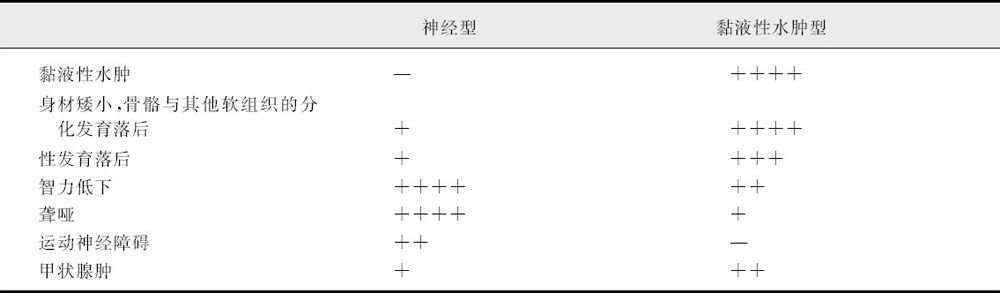
\includegraphics{./images/Image00014.jpg}
\end{table}

除了明显的甲状腺功能减退和甲状腺肿外,还存在着许多亚临床病人。De
Quarrain与Wegelin首先用类甲状腺功能减退症来描述亚临床病人,并做如下规定:如有可疑甲状腺功能低下、可疑智力低下或两者均有,只要有其中一项,则考虑为类甲状腺功能减退症。亚临床体格发育落后症候群:主要是身高和体重低于正常儿童,某些生理检查指标如握力、肺活量和血压等也偏低,少数人还有轻度骨骺发育落后,性发育落后一般不明显。

(四)营养状况评价

{1.尿碘}
 习惯上根据尿碘的排出量来评价机体碘的营养状况,儿童尿碘<100μg/24h,提示碘营养不良。

{2.激素水平}  包括T\textsubscript{3} 、FT\textsubscript{3}
、T\textsubscript{4} 、FT\textsubscript{4}
、TSH的水平,其中T\textsubscript{3} 稍高,T\textsubscript{4}
、FT\textsubscript{4} 下降,TSH升高是碘缺乏的表现。

{3.儿童甲状腺肿大发生率}
 如甲状腺肿大发生率>5%,则提示碘营养不良,但甲状腺肿可能是过去碘缺乏所造成,碘缺乏予以纠正以后,甲状腺肿可能需数月甚至数年才能消退,而尿碘则在正常水平。

(五)诊断

{1.地方性甲状腺肿}

我国制定的诊断标准有3条:

(1)居住在碘缺乏地区。

(2)甲状腺肿大超过受检者拇指末节,或小于拇指末节而有结节者。

(3)排除其他甲状腺疾病,如甲亢、甲状腺炎和甲状腺癌等。此外,实验室检查表现为尿碘偏低,血浆中TSH可有不同程度增高,血浆中T\textsubscript{4}
、T\textsubscript{3} 浓度多属于正常,但严重病人T\textsubscript{4}
低于正常、T\textsubscript{3}
稍高,甲状腺扫描也可见弥漫型或结节性甲状腺肿大。

{2.地方性克汀病的诊断标准}

(1)出生、居住于低碘地方性甲状腺肿病地区。

(2)有精神、神经发育不全,主要表现为不同程度的智力障碍、语言障碍和运动神经障碍。

(3)不同程度的体格和性发育障碍,特殊的典型面容。

(4)辅助检查 包括T\textsubscript{3} 、T\textsubscript{4}
、TSH的水平异常。X线表现为骨龄落后,以成骨中心及骨骺不能按时出现为多见,颅骨脑回压迹增多,颅底短小,蝶鞍偶见增大。

如具有上述任何一项症状或体征,再加上一项辅助检查指标为阳性者,而又可排除分娩损伤、脑炎、脑膜炎及药物中毒等病史者,即可诊断为地方性克汀病。

(六)预防和治疗

{1.去除病因}
 首先去除病因,由于膳食因素引起,应先调整饮食,如为药物引起,要停药或换另1种药物代替。

{2.饮食疗法}
 每天碘的推荐摄入量3岁以内的儿童为50μg,7~10岁的儿童为90μg,11~17岁为120~150μg,成人为150μg;孕妇和乳母为200μg。如碘摄入不足,可适当补充含碘量高的食物,海产品中碘的含量较高,如海带、紫菜、干贝等。食盐中加碘也是防治碘缺乏的重要措施,进入用户的食盐中碘比例1∶50000(含量不得<20mg/kg)可有效地预防地方性甲状腺肿,1∶20000(含量为50mg/kg)可预防地方性甲状腺功能减退症。现在我国大部分地区,食盐中已经加碘,明显减少了碘缺乏病的发生率。

{3.药物治疗}
 可通过碘化油的口服或注射来满足机体对碘的需要。碘化油是一种长效、经济、方便、不良反应少的防治药物,目前常用的是巴黎Guerter实验室的产品,名为Lipodol
UF的产品用于肌注,Oridol的产品用于口服。但在剂量方面,仍存在分歧。根据缺碘的程度和具体条件予以补充,一般来说,推荐剂量是1ml,每6个月需重复1次口服剂量。如补碘后,甲状腺肿大仍不能控制,可采用甲状腺制剂治疗,以补充内源性甲状腺激素不足,可使甲状腺减小或消失。

{4.手术治疗}
 一般不采取手术治疗,但甲状腺肿大严重,引起压迫症状,且内科治疗无效者,可行手术治疗。

\hypertarget{text00003.htmlux5cux23mllj25}{%
\section{ 营养性贫血}\label{text00003.htmlux5cux23mllj25}}

\hypertarget{text00003.htmlux5cux23mllj26}{%
\subsection{缺铁性贫血}\label{text00003.htmlux5cux23mllj26}}

作为人体所需的微量元素铁不仅是血色素分子的组成部分,在氧和电子输送中起着核心作用,也是肌红蛋白、骨骼肌和脑等细胞中的一系列氧化脱氢酶所不可缺少的组成部分,另外还参与一些具有清除、中和有毒基团及化学物质的铁依赖性酶的合成,在免疫防御中起重要作用。铁缺乏性贫血(iron
deficiency anemia,
IDA)是遍及全世界的最常见的营养缺乏症,以出生后6个月至3岁的小儿发生率最高,但根据1994年调查结果显示,在美国仍有9%的<3岁的小儿存在着铁的缺乏,其中1/3患有缺铁性贫血。1995年我国报道发生率很高,上海地区<2岁的婴幼儿缺铁性贫血发生率为32%;全国<3岁的达50%,主要原因是膳食营养不平衡、膳食中铁摄入量不足引起。2002年北京报道该市顺义区12个月以前的婴儿缺铁性贫血的发生率仍达30%。我国第三次全国营养调查显示,我国成年女性IDA患病率城市和乡村分别为23.5%和26.2%;2002年我国第四次营养调查显示,我国居民贫血发生率为20.1%,男性15.8%,女性23.3%;城市和乡村分别为21.5%和24.0%,2岁以下婴儿和60岁以上的老年人分别为31.1%和29.1%。

(一)缺铁的分期

缺铁(iron
deficiency)是指机体含铁量低于正常。根据铁耗竭的不同阶段理论上可分为以下3期。

{1.铁减少期(iron depletion, ID)}
 本期为缺铁的最早期,也称隐匿前期,此期仅有储存铁减少,除骨髓细胞外铁减少、血清铁蛋白低于正常外,其他如骨髓铁粒幼细胞、血清铁、转铁蛋白饱和度、血红蛋白等均正常。

{2.红细胞生成缺铁期(iron deficiency erythropoiesis, IDE)}
 也称为无贫血缺铁期,此期特点为储存铁减少或消失,血清铁蛋白低于正常,骨髓铁粒幼细胞减少(一般<10%),红细胞原卟啉高于正常,血清铁及转铁蛋白饱和度可降低,总铁结合力可增高,但血红蛋白及红细胞比容正常,红细胞为正色素。

{3.缺铁性贫血期(iron deficiency anemia, IDA)}
 除上述指标异常外,血红蛋白或红细胞比容也下降,出现不同程度的低色素性贫血。

(二)缺铁对机体的影响

体内含铁化合物中,血红蛋白及肌红蛋白具有带氧功能,细胞色素、琥珀酸脱氢酶及NADH脱氢酶等能运送电子,过氧化氢酶能分解过氧化氢。铁除包含在上述含铁化合物中外,尚与很多酶的活性有关,如单胺氧化酶、酪氨酸羟化酶、核糖核苷酸还原酶等,此类酶控制着体内主要的氧化、水解和转运过程。因此,铁与组织呼吸、氧化磷酸化、卟啉代谢、胶原合成、淋巴细胞与粒细胞功能、神经介质的合成与分解、躯体与神经组织的发育都有密切关系。

{1.对造血系统的影响}
 铁是合成血红蛋白的原料。血浆中转运的铁到达骨髓造血组织时,铁即进入幼红细胞内,被线粒体摄取与卟啉结合而形成正铁血红素,后者再与珠蛋白合成血红蛋白。当体内缺铁时,正铁血红素形成不足,使血红蛋白合成减少,新生的红细胞中血红蛋白量不足。明显缺铁时,由于影响到DNA的合成,对幼红细胞的分裂增殖也有一定影响,但远不如对血红蛋白合成的影响明显,故新生的红细胞体积变小,胞质中血红蛋白减少,而形成小细胞性低色素性的贫血。临床表现有乏力、心慌、气短、头晕、眼花,严重者出现面色、口唇黏膜和睑结膜苍白、肝脾轻度肿大等,继发贫血性心脏病时易发生左心衰竭。

{2.对精神运动系统和生长发育的影响}
 大量研究已证明,缺铁最主要的影响是不利于儿童的行为和生长发育。缺铁可能是行为异常,如易怒、注意力不集中等的原因。患有缺铁性贫血的婴儿和儿童存在着明显的精神运动测试的障碍,在某种程度上能通过铁剂治疗被纠正,而相当一部分患儿已不能用铁剂来逆转,婴幼儿期如果患了较严重的缺铁性贫血,虽经积极补铁纠正,到儿童期的智商测定结果仍低于正常儿童,所以强调预防铁营养缺乏而致的不可逆性的精神运动是至关重要的。小儿在缺铁时还可出现屏气发作,待纠正后屏气发作即会消失。有些铁缺乏病人有噬食泥土、煤炭、石灰、墙泥、生米等异食癖,用铁剂治疗后这些异食行为可以消失。

另外,铁缺乏将促使铅中毒,动物和人的研究证明严重铁缺乏常伴有胃肠道铅的吸收上升,而且吸收入体内的铅又抑制铁络合酶,阻止铁与原卟啉的络合过程,使原卟啉在体内堆积,使血红蛋白的合成更加减少。临床和流行病学调查结果也显示了血铅水平和缺铁的相关性。由于铅中毒是神经系统和儿童发育障碍的主要原因,故铁缺乏又直接或间接地通过增加铅的吸收而促成这一病变。

{3.对消化系统的影响}
 严重缺铁可致黏膜组织变化和外胚叶组织营养障碍,可表现为胃酸减少、口腔黏膜异常角化和变薄、色素减退,可发生萎缩性舌炎和胃炎,吞咽困难,小肠黏膜绒毛可变宽、变钝、融合,上皮下可有炎症。胃活检发现75%的缺铁性贫血病人可呈表浅性胃炎和不同程度的萎缩性胃炎的病理改变,而对照组仅为29%;在小儿甚至可产生渗出性病变和吸收不良综合征,导致脂肪泻等。

{4.对免疫系统功能的影响}
 近年来,很多研究证实缺铁时,与杀菌有关的很多含铁酶或依赖铁的酶活性明显下降;铁还可直接影响淋巴组织的发育和对感染的抵抗力;抗原刺激后淋巴细胞转化率及巨噬细胞移动抑制因子的产生均下降;中性粒细胞吞噬功能降低,皮肤过敏试验应答下降,对细胞免疫功能有一定程度的损害。缺铁易引起感染、疲劳、倦怠、工作效率和学习能力降低,使机体处于亚健康状态。

另有作者从临床和实验证明缺铁性贫血病人的抵抗力和细胞免疫反应等均正常,在试管和动物实验中,加入铁元素能促进细菌和白色念珠菌等繁殖和毒力增强,用转铁蛋白螯合后又可抑制细菌繁殖。因此,临床上大剂量补铁时要慎重。

(三)实验室检查

{1.生化方法}

(1)血清铁蛋白(serum ferritin,
SF):反应体内铁储存的1个较正确和灵敏的指标,体内缺铁时SF下降,当SF<12μg/L时表明机体已处于缺铁状态。

(2)红细胞内游离原卟啉(free erythrocyte protoporphyrin,
FEP):正常值为500μg/L,IDE或IDA时FEP上升,FEP/Hb较敏感,其比值>3μg/g则考虑为异常,若在5.5~17.5μg/g范围内,如能排除铅中毒,即可诊断为缺铁性贫血,在美国常作为筛查铁缺乏的手段。

(3)血清铁(serum iron, SI):常降低(正常值:8.95~21.48μmol/L)。

(4)运铁蛋白(transferrin,
TF):正常成人2~4g/L,初生时低,2个月后逐渐上升,至2岁达成人水平。

(5)总铁结合力(total iron binding capacity,
TIBC):常上升(正常值为54~64μmol/L)。

(6)运铁蛋白饱和度(transferrin saturation,
TS):常下降至15%以下(正常值为35%~40%),炎症时也可下降,但与铁缺乏不同,总铁结合力也下降。

{2.血象}
 血红蛋白(Hb)较红细胞计数(RBC)减低更明显,故红细胞平均容积(MCV)、红细胞平均血红蛋白量(MCH)较正常为小或低。红细胞平均血红蛋白浓度(MCHC)正常或下降。

{3.其他}
 肝细胞储铁和组织含铁量以及铁吸收和铁动力学等的测定,但这些都不实用或不敏感,不能常规应用。

(四)诊断标准

为提高对铁缺乏和缺铁性贫血诊断的准确性,国内外都制定了相应的诊断标准。1982年全国小儿血液病学学术会议(洛阳)提出小儿铁缺乏的诊断标准,而对国内成人尚缺乏统一的诊断标准。

{1.缺铁性贫血(IDA)的诊断标准}

(1)男性Hb<130g/L,女性Hb<120g/L,孕妇Hb<110g/L;MCV<80fl,
MCH<26pg, MCHC<310g/L;红细胞形态有明显低色素表现。

(2)有明显的缺铁病因和临床表现。

(3)血清铁(SI)<10.7μmol/L,总铁结合力(TIBC)>64.4μmol/L。

(4)血清运铁蛋白饱和度(TS)<15%。

(5)骨髓铁染色显示骨髓小粒可染铁消失,铁粒幼红细胞<15%。

(6)红细胞游离原卟啉(FEP)>0.9μmol/L(全血),或血液锌原卟啉(ZPP)>0.96μmol/L(全血),或FEP/Hb>4.5μg/gHb。

(7)血清铁蛋白(SF)<14μg/L。

(8)铁剂治疗有效。

符合第(1)条和(2)~(8)条中任何2条以上者可诊断为缺铁性贫血。

{2.铁缺少期(ID)的诊断标准}

(1)血清铁蛋白(SF)<14μg/L。

(2)骨髓铁染色显示骨髓小粒可染铁消失。

符合以上任何1条即可诊断为贮存铁缺乏期。

{3.红细胞生成缺铁期(IDE)的诊断标准}

(1)血清运铁蛋白饱和度(TS)<15%。

(2)红细胞游离原卟啉(FEP)>0.9μmol/L(全血),或血液锌原卟啉(ZPP)>0.96μmol/L(全血),或FEP/Hb>4.5μg/gHb。

(3)骨髓铁染色显示骨髓小粒可染铁消失,铁粒幼红细胞<15%。

符合贮存铁缺乏期的诊断标准,同时又有以上任何1条即可诊断为红细胞生成缺铁期。

{4.WHO制定的铁缺乏诊断标准}
 血清铁(SI)<8.95μmol/L,血清运铁蛋白饱和度(TS)<15%,血清铁蛋白(SF)<12μg/L,红细胞游离原卟啉(FEP)>1.26μmol/L。

(五)治疗和预防

{1.去除病因}
 查明缺铁原因,除膳食中铁不足外,还需注意钩虫和消化道隐性出血性疾病的存在。

{2.饮食疗法}
 增加膳食含铁量并注意合理配合,补充含血红素丰富的红色肉类、动物肝脏和血液等。母乳中含铁量虽不高(0.3~0.5mg/L),但吸收率高达50%;血红素含铁高(3.4mg铁/g),其吸收率也较高(10%~26%);黄豆比其他植物类食物的含铁量高(11mg铁/100g),吸收率也有7%,上述食品和铁强化食品(1L奶中含铁12mg,1kg面粉中含铁13~15mg)是较理想的防治缺铁的食品。

{3.铁剂治疗}

(1)口服:常用制剂有硫酸亚铁、富马酸铁、葡萄糖酸亚铁、琥珀酸亚铁、柠檬酸铁胺等。剂量为元素铁4.5~6mg/(kg·d),一般治疗后3~4周有效,可维持巩固4~8周。同时服用维生素C可使铁吸收率增加3倍。不良反应有食欲下降、恶心、呕吐、腹痛、腹泻等。

(2)肠外途径应用:需严格掌握应用指征:①口服有严重不能耐受的不良反应;②长期腹泻、呕吐或大部分小肠切除后需要全肠外营养维持者。右旋糖酐铁含铁量50mg/ml,总补铁量的计算公式:

总补铁量(mg)=体重(kg)×[Hb目标值-Hb实际值](g/L)×0.238+贮存铁量(mg)

贮存铁量=10mg/kg 体重(<700mg)

肌注时每1~3天注射1次,首次可用12.5~25mg,若无不良反应,再增加至50mg,直至总量用完。现实验研究已得到肯定,右旋糖酐铁可以加入TPN混合液中进行输注。足月新生儿一般出生后4个月内,不需额外补充外源性铁,然而早产或低出生体重儿由于在胎儿期铁贮存有限,需要提前给予补充,James等建议小儿剂量为0.7mg/(kg·d)。Friel等也对一种小儿多种微量元素制剂(Ped
EL,
Pharmacia产品)进行了评价,在一组平均体重为910g的超低出生体重儿中,给予铁120μg/(kg·d),平均可使体内储存铁930μg/(kg·L)。对于低出生体重儿和极低出生体重儿,虽然精确的应用剂量没有确定,但补充的最终目的应该允许储存铁达到足月新生儿在胎儿期通过胎盘所得到的铁的储存量。目前有全量补充法和小剂量每天或周期性(隔天或每周1次)补充法两种,前者往往用于铁严重耗竭或严重缺铁性贫血者,后者用于轻度铁缺乏或作为一般生理量的维持。

静脉应用的不良反应有局部疼痛、局部皮肤变色、面部潮红、头痛、肌肉关节痛、腹痛、呕吐、腹泻、发热、淋巴结肿大,偶有心律紊乱、惊厥和过敏性休克。低剂量应用尚无过敏反应报道,而对于快速输注(25mg/100ml葡萄糖液)会引起严重变态反应的病人,改用1~2mg/d右旋糖酐铁常规维持还是成功的。

静脉补充时的注意事项:①在全量补充法前,先予小剂量5mg(0.1ml静脉输注)试验来筛查过敏者。在全量补充时,需备有复苏设备和包括麻醉师在内的一组技术熟练的急救成员以防意外。②肠外途径补充铁剂,不能忽视小肠对机体铁需要量的调节作用,小肠不仅吸收铁,而且也是排泄铁的重要器官,故长期应用添加铁剂的广泛小肠切除的TPN支持病人,应注意其血清铁的生化监测,避免和防止铁负荷过多或铁中毒。③有潜在的促使铁依赖性病原体感染的播散作用,有报道新生儿肌注右旋糖酐铁可增加败血症的发生率。

\hypertarget{text00003.htmlux5cux23mllj27}{%
\subsection{营养性巨幼红细胞性贫血}\label{text00003.htmlux5cux23mllj27}}

巨幼红细胞性贫血又称为营养性大细胞性贫血(megaloblatic
anemia),是由于维生素B\textsubscript{12}
及叶酸缺乏,导致脱氧核糖核酸(DNA)合成障碍所引起的贫血。外周血的红细胞平均容积(MCV)和平均血红蛋白(MCH)均高于正常。叶酸、维生素B\textsubscript{12}
都属于水溶性维生素,维生素B\textsubscript{12}
是一种可以预防和治疗由于内因子缺乏活性以致吸收障碍而引起的恶性贫血的维生素。在我国各地,因叶酸缺乏所致的巨幼红细胞性贫血比维生素B\textsubscript{12}
缺乏多见。

(一)病因

{1.摄入不足,需要量增加}  FAO/WHO推荐正常成人维生素B\textsubscript{12}
需要量为每天1μg/d,我国目前提出的适宜摄入量(AI)0~3岁为0.4~0.9μg/d,4~7岁为1.2~1.8μg/d,成人为2.4μg/d。2000年我国营养学会推荐每天叶酸摄入量(RNI)为400μg,0~6个月为65μg(AI),7~12个月为80μg(AI),1~12岁为150~300μg,13岁以上至成人为400μg,妊娠期为600μg,哺乳期为500μg。未成熟儿、新生儿及婴儿期生长发育迅速,造血物质需要量相对增加,如摄入不足,则易缺乏。消毒奶类时,可使叶酸破坏,出生时低出生体重儿于生后6~10周时即发病。在怀孕和生长发育期及患溶血性贫血、白血病、恶性肿瘤等疾病,叶酸的需要量增加3~6倍,如果不及时补充,会造成叶酸缺乏,4个月后则会出现巨幼红细胞性贫血。

{2.吸收障碍}  恶性贫血存在内因子抗体,阻止了维生素B\textsubscript{12}
与内因子结合;胃黏膜萎缩,也造成了内因子缺乏;小肠疾病,如短肠综合征等,常同时有叶酸和铁的吸收减少。

{3.先天贮存不足}  胎儿可通过胎盘,获得维生素B\textsubscript{12}
、叶酸贮存在肝脏中,如孕妇患维生素B\textsubscript{12}
或叶酸缺乏时则新生儿贮存少,易发生缺乏。

{4.疾病因素}  感染、疟疾及慢性溶血时,需要量增加,感染又影响吸收。

{5.维生素C缺乏}
 维生素C缺乏时,不能使叶酸变为具有活性的四氢叶酸(tetrahydrofolic acid,
THFA)。叶酸能代替维生素C参与酪氨酸代谢,当维生素C缺乏时,可引起机体对叶酸的需要量增加,造成叶酸不足。

(二)发病机制

叶酸和维生素B\textsubscript{12}
均为细胞核内DNA合成的必需物质。细胞的增殖分裂,关键是DNA的复制。DNA是由2条多核苷酸链组成,其基本单位是由4种不同的碱基单核苷酸组成的聚合体,4种碱基为腺嘌呤、鸟嘌呤、胸腺嘧啶和胞嘧啶。

叶酸在肝内经二氢叶酸还原酶的作用,变为具有活性的THFA。THFA是体内转移一碳基团的辅酶。这些基团来自一些氨基酸的分解代谢和甲酸等化合物,可连接在THFA的分子上,并可转移至其他中间代谢物上,参与核酸等重要化合物的合成,如参与嘌呤的合成、嘧啶的生物合成、氨基酸的转化以及甲酸盐的生成和利用。

维生素B\textsubscript{12}
在人体主要参与4个重要代谢反应:①使无活性的甲基THFA变为有活性的THFA,提高了叶酸利用率。②促进叶酸进入细胞内。③参与脱氧胸腺嘧啶核苷酸的生成。由上可见,维生素B\textsubscript{12}
缺乏是通过叶酸代谢障碍,引起DNA合成失常,故其引起贫血的临床表现和形态学变化,难与叶酸缺乏引起的贫血区别。这说明为什么维生素B\textsubscript{12}
可使叶酸缺乏的贫血好转,以及大量叶酸能改变维生素B\textsubscript{12}
缺乏的血液学变化的现象。④维生素B\textsubscript{12}
能促使脂肪代谢产物参与三羧酸循环,这一作用与神经髓鞘中脂蛋白的形成有关,因而能保持中枢和外周有髓鞘的神经纤维的完整功能。维生素B\textsubscript{12}
缺乏时,上述神经纤维发生病变,因而出现精神神经症状。因叶酸不参与此代谢,不能改变维生素B\textsubscript{12}
缺乏所致的神经系统损害。不过叶酸增加可导致造血细胞对维生素B\textsubscript{12}
的利用,神经系统需要的维生素B\textsubscript{12}
相应减少,故可加剧神经系统的症状。

叶酸和维生素B\textsubscript{12}
缺乏时,嘌呤和胸腺嘧啶合成不足,DNA复制受阻。在DNA复制时由于α聚合酶的活力显著降低,使新合成的DNA短片在形成长链时发生障碍,在重螺旋化时易受机械损伤、染色体断裂、细胞死亡而形成无效造血。DNA合成障碍也使细胞分裂受阻、DNA含量多,加之螺旋化不佳,故呈现细胞核大、染色质网状结构。同时由于蛋白质及RNA合成相对较好,而导致胞质量多、核浆发育不平衡的巨幼样变。此变化也累及骨髓中的粒细胞和巨核细胞系统及体内细胞代谢快速。

(三)临床表现

{1.一般症状}
 发病一般缓慢,轻者仅皮肤、黏膜苍白而无自觉症状,逐渐出现乏力、倦怠、头晕、心悸等。

小儿病例初起时表现安静,不哭不闹。面色逐渐苍白或因色素过度沉着、轻度贫血等因素,面色可为蜡黄。睑结膜、口唇明显苍白,头发细黄且稀疏,颜面有水肿,成人病例可有头昏、耳鸣、心慌等。通常从4~6个月开始,而以9~18个月多见,若出生时为早产儿,则由于其先天的叶酸贮存量较少、生长发育快、尿中的排出量相对较多,又由于奶类消毒后,叶酸破坏、进入量较少,所以出生体重较轻者可于出生后6~10周即发病。

{2.消化系统症状}
 出现较早,由于消化道黏膜上皮细胞DNA合成障碍可产生一系列症状,如厌食、恶心、呕吐较常见,时有稀便,舌面可光滑,舌乳头由舌尖沿两侧缘逐渐向中心萎缩,或舌乳头充血粗糙等。

{3.造血系统表现}
 肝肿大远较脾肿大为多,肿大程度亦较脾脏为著,淋巴结肿大不明显。由于成熟红细胞寿命短,可有轻度黄疸、口唇、甲床和睑结膜等处明显苍白。同时可有白细胞和血小板减少,常有感染和出血倾向,如紫癜、鼻出血、月经过多等现象。

{4.神经精神方面症状}
 小儿较成人常见。有表情呆滞、眼神发直、对周围反应迟钝,嗜睡、智力及动作能力均可有倒退。由于维生素B\textsubscript{12}
缺乏,脊髓髓质合成障碍,侧索、末梢神经等均可受到损害,因此可发生手足对称性麻木、感觉障碍、共济失调、步态不稳、行走困难、腱反射亢进等。少数病例可能由于9、10对颅神经功能障碍而出现声音嘶哑或咽部有痰声。自主神经系统受累时,可出现少泪、无泪、少汗等症状,此症状多见于维生素B\textsubscript{12}
缺乏。

{5.其他循环症状}
 比缺铁性贫血为显著,心前区可听到功能性收缩期杂音的达60%~70%,心脏扩大,易引起心功能不全。

(四)诊断

巨幼红细胞性贫血的诊断依据:骨髓中出现较多典型巨幼红细胞,平均红细胞体积(MCV)>95
μm\textsuperscript{3}
,卵圆形大红细胞增多,明显的大小不均和异形,中性粒细胞分叶过多等。巨幼红细胞性贫血诊断成立后必须进一步明确是叶酸缺乏还是维生素B\textsubscript{12}
缺乏。用血液形态学的检验方法是无法区别的。根据病史、体征、特殊实验室检查,可加以鉴别(表2-6)。

表2-6 叶酸与维生素B\textsubscript{12}
缺乏所致巨幼红细胞性贫血的鉴别诊断

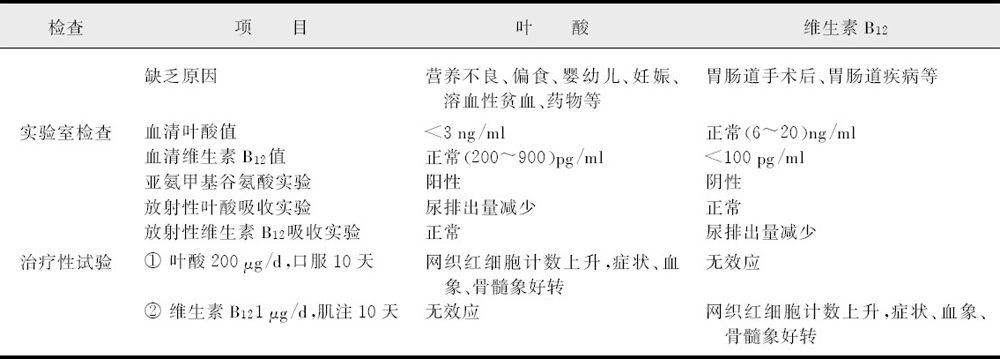
\includegraphics{./images/Image00015.jpg}

(五)预防和治疗

{1.预防}
 预防本病应从改善人群膳食结构入手,对易发病个体应提高药物预防意识。大多数病例的叶酸和维生素B\textsubscript{12}
的缺乏是可以预防的。如为母乳喂养儿,应改善乳母的膳食营养,婴儿还须添加辅食。积极预防和治疗呼吸道和消化道疾病。改变不良的饮食习惯,尤其要做到不偏食、不挑食和不长期素食。从食物中摄取足够的叶酸和维生素B\textsubscript{12}
。去除病因,改善营养状况和饮食的食物组成,是保证不再复发的重要措施。

{2.供给富含叶酸和维生素B\textsubscript{12} 的食物}
 每天从膳食中至少要摄取50~100μg叶酸含量的食物,富含叶酸的食物有动物肝脏、内脏类、西红柿、莴苣、菠菜、油菜、小白菜、芦笋、豆类及发酵制品(如腐乳、豆豉等)、麦麸、全麦、深绿色蔬菜及酵母等。含维生素B\textsubscript{12}
丰富的食物有动物肝、肾和肉类,蛋类,牛乳,面粉,蔬菜中也含有少量维生素B\textsubscript{12}
。此外,橘子汁含有丰富的维生素C和叶酸,一杯橘子汁约含叶酸50μg。如为母乳喂养儿,应改善乳母的膳食营养,婴儿还须添加辅食。积极预防和治疗呼吸道和消化道疾病。

{3.药物治疗}  如明确系叶酸或维生素B\textsubscript{12}
缺乏时,可给相应药物治疗。如不明确时,神经系统症状以应用维生素B\textsubscript{12}
的收效较佳,单用叶酸反有加重症状的可能。若同时有维生素B\textsubscript{12}
及叶酸的缺乏,应用其中的1种有可能使另1种更为缺乏,故宜两药同时应用。

(1)叶酸:剂量为5~10mg/d,治疗后1~2天食欲、精神即改善,无效红细胞生成逆转,网织红细胞逐渐上升,至4~7天达高峰,于2~6周后恢复正常。治疗后24~48小时,白细胞及血小板计数即上升。骨髓中除巨晚幼粒等细胞可持续存在数天外,于治疗48小时后已很少有其他变化。叶酸的疗程常需数月,即用至体内年老红细胞均被新生富有叶酸的红细胞替代为止。去除病因及改善饮食是保证不再复发的重要措施。服用叶酸的同时需服用维生素C。

(2)维生素B\textsubscript{12}
:剂量为25~100μg/次,症状严重时可每天1次肌注,否则可每周2~3次肌注,至网织红细胞恢复正常时为止。如病因暂时不能去除,则需减量,维持至红细胞及血红蛋白恢复正常而停药。血及骨髓象的恢复过程与叶酸缺乏相似,神经系统症状恢复较慢。

{4.补充富含维生素C的食物}
 维生素C能促进叶酸的吸收,在维生素C缺乏时,叶酸的吸收率下降。应多吃富含维生素C的新鲜蔬菜和水果。但维生素C的补充量不宜过大,如>500mg,就会使维生素B\textsubscript{12}
进一步缺乏。

(六)预后

营养性巨幼红细胞性贫血在应用维生素B\textsubscript{12}
治疗后预后良好。在给药2~3天后可见精神好转,对周围环境反应逐渐灵敏,此后食欲转佳。但是,震颤消失减慢,大多需要1个月以上。少数病例在治疗过程中震颤加重,终能消失。但是,治疗晚的可影响小儿的智力发育。

\hypertarget{text00003.htmlux5cux23mllj28}{%
\subsection{维生素缺乏与贫血}\label{text00003.htmlux5cux23mllj28}}

(一)维生素C缺乏

维生素C缺乏时,叶酸在体内还原为具有生物活性的四氢叶酸受阻。叶酸能代替维生素C参与酪氨酸代谢,维生素C缺乏时,叶酸需要量增加。由于以上两个方面的原因,维生素C缺乏可引起巨幼红细胞性贫血。维生素C缺乏引起贫血的另1个原因是出血。

(二)维生素E缺乏

维生素E缺乏多发生在早产儿及低出生体重儿,尤其在出生体重<1500g者易见。其原因有摄入不足、吸收不良、运转维生素E的脂蛋白量降低、生长发育迅速时,维生素E的需要量增加,食物中含有大量不饱和脂肪酸,饮食中不饱和脂肪酸的增加,可增加红细胞膜不饱和脂肪酸的含量。维生素E为抗氧化剂,有防止红细胞膜上不饱和脂肪酸被氧化的作用。维生素E缺乏时,红细胞膜上脂质易被氧化,尤其在遇到过氧化氢、巴比妥酸、维生素K及低出生体重儿服用较大量铁剂以预防缺铁性贫血时。本症常发生在早产儿和低出生体重儿,尤其是人工喂养者,于出生后6~10周出现维生素E缺乏综合征,症状包括不安宁、惊醒、水肿、轻度溶血等。血红蛋白可低至70~90g/L,红细胞大小不均、异形、破碎细胞,偶有球形,血小板常增多,过氧化氢试验呈阳性,维生素E测定常<10μmol/L。正常婴儿维生素E的需要量各人报道并不一致。用乳类喂养者为0.4mg/d,用其他食物喂养者为1.5mg/d。早产儿的维生素E含量明显低于足月儿,至出生后2~3个月,早产儿肠道吸收的量已达到足月儿水平,维生素E含量才升高。由于维生素E缺乏而引起的严重贫血并不常见,但为了尽量减少此病的发生,对低出生体重儿应给予维生素E以作预防,剂量为15~25mg/d,出生体重<1000g者增加到50mg/d,可使维生素E维持到正常水平。有胰腺囊性纤维化和慢性脂肪吸收不良的患儿,应增加到100mg/d。肌注比口服效果好。肌注为隔天1次,共用2~3次。

(三)其他维生素缺乏与贫血

其他维生素缺乏也可引起贫血,如维生素A、维生素B\textsubscript{2}
缺乏。另有原因不明的维生素B\textsubscript{1}
反应性巨幼红细胞性贫血。维生素B\textsubscript{6}
参与δ-ALA合成酶的代谢,缺乏时血红素合成发生障碍,出现小细胞性低色素性贫血,临床上极少见。另1种维生素B\textsubscript{6}
反应性贫血(小细胞性低色素性),能被大剂量维生素B\textsubscript{6}
所纠正,其发病机制可能为线粒体内铁的利用障碍,血红素离开线粒体时需要维生素B\textsubscript{6}
的作用。尼克酸缺乏时(由于腹泻等)可引起贫血。

{参考文献}

[1]葛可佑.中国营养科学全书.北京:人民卫生出版社,2004,1431~1444

[2]滕红红,王晓华,李辉,等.2000~2004年中国儿童维生素A缺乏状况研究.中国儿童保健杂志,2006,14(3):270~271

[3]蔡美琴.医学营养学.第二版.上海:上海科学技术出版社,2007

[4]诸福堂.实用儿科学.第七版.北京:人民卫生出版社,2002,508~558

[5]Ronald E. Pediatric Nutrition Handbook. 6th ed. America: America
Academy of Pediatrics, 2009, 559~576

[6]Gautam B, Deb K, Banerjee M, Serum zinc and copper level in
children with protein energy malnutrition. Mymensingh Med J, 2008, 17
(2Suppl): S12~S15

[7]Orwoll E, Nielson CM, Marshall LM, et al.Vitamin D deficiency in
older men. J Clin Endocrinol Metab, 2009, 94 (4): 1214~1222

\protect\hypertarget{text00004.html}{}{}

